\documentclass[12pt,spanish]{article}
\usepackage[spanish]{babel}
\usepackage{graphicx}
\usepackage{color}
\usepackage{xcolor}
\usepackage{colortbl}
\usepackage{multirow}
\usepackage{amsmath}
\usepackage{subcaption}
\usepackage{adjustbox}
\usepackage{multirow}
\usepackage[hidelinks]{hyperref}
\usepackage{caption}
\usepackage{amsthm}
\usepackage{multicol}
\usepackage[outputdir=build]{minted}
\usepackage{float}
\usepackage{titling}
\usepackage{soul}
\usepackage{listings}
\usepackage{array}
\graphicspath{ {./img/} {../../LaTeX/img/}}
\selectlanguage{spanish}
\usepackage[utf8]{inputenc}
\usepackage{graphicx}
\usepackage[a4paper,left=2cm,right=2cm,top=2.5cm,bottom=2.5cm]{geometry}


\title{Arquitectura de Computadores}
\setlength{\droptitle}{10em}
\author{Carlos Sánchez Páez}

\makeindex
\begin{document}


\begin{titlepage}

\newlength{\centeroffset}
\setlength{\centeroffset}{-0.5\oddsidemargin}
\addtolength{\centeroffset}{0.5\evensidemargin}
\thispagestyle{empty}

\noindent\hspace*{\centeroffset}
\begin{minipage}{\textwidth}

\centering

\includegraphics[width=0.9\textwidth]{logo_ugr.jpg}\\[1.4cm]

\textsc{ \Large Fundamentos de Ingeniería del Software\\[0.2cm]}
\textsc{GRADO EN INGENIERÍA INFORMÁTICA}\\[1cm]

{\Huge\bfseries Resumen del temario\\}
\end{minipage}

\vspace{1.5cm}
\noindent\hspace*{\centeroffset}
\begin{minipage}{\textwidth}
\centering

\textbf{Autor}\\ {Carlos Sánchez Páez}\\[2.5ex]

\includegraphics[width=0.3\textwidth]{etsiit_logo.png}\\[0.1cm]
\vspace{1.5cm}

\includegraphics[width=0.2\textwidth]{lsi.png}\\[0.1cm]
\vspace{1cm}
\textsc{Escuela Técnica Superior de Ingenierías Informática y de Telecomunicación}\\
\vspace{1cm}
\textsc{Curso 2017-2018}
\end{minipage}
\end{titlepage}
\thispagestyle{empty}
\newpage
\tableofcontents{}
\newpage
\listoffigures
\thispagestyle{empty}
\newpage

\section{Tema 1. Introducción a la Ingeniería del Software}

\subsection{El producto Software}

\subsubsection{Definición de Software}

El software se puede definir de varias formas:
\begin{itemize}
\item Programa o conjunto de programas de cómputo que incluye datos, procedimientos y pautas que permiten realizar distintas tareas en un sistema informático.
\item Transformador de información, para lo que adquiere, gestiona, modifica, produce o transmite esa información.
\end{itemize}

\subsubsection{Tipos de software}

Podemos clasificar el software en varios tipos:
\begin{enumerate}
	\item Por \emph{campo de aplicación}:
		\begin{enumerate}
			\item Software de \textbf{sistemas}.
			\item Software de \textbf{aplicaciones}.
			\item Sotware de \textbf{programación}.
		\end{enumerate}
	\item Por \emph{tipo de licencia}:
		\begin{enumerate}
			\item Según derechos de autor
				\begin{enumerate}
					\item Software de \textbf{código abierto}.
					\item Software de \textbf{código cerrado}.
					\item Software de \textbf{dominio público}.
				\end{enumerate}
			\item Según su destinatario
				\begin{enumerate}
					\item Usuario final (software \textbf{hecho a medida}).
					\item Para distribución (software \textbf{genérico}).
				\end{enumerate}
		\end{enumerate}
\end{enumerate}

\subsubsection{Características principales}

\begin{enumerate}
	\item El software es un producto lógico:
		\begin{enumerate}
			\item No se fabrica, sino que se desarrolla.
			\item No se estropea, sino que se deteriora.
		\end{enumerate}
	\item Crea modelos de la realidad.
	\item Está formado por múltiples piezas que deben encajar perfectamente.
\end{enumerate}

\subsubsection{Proceso de producción}

El proceso de producción del software está formado por las siguientes etapas:
\begin{enumerate}
	\item \textbf{Definición}. Debemos precisar lo que queremos desarrollar. Para ello debemos realizar varias tareas:
		\begin{itemize}
			\item Ingeniería de Sistemas.
			\item Ingeniería de Requisitos.
			\item Planificación de proyectos.
		\end{itemize}
	\item \textbf{Construcción}. Hemos de determinar cómo desarrollaremos el software. Depende de:
		\begin{itemize}
			\item Diseño del software.
			\item Generación del código.
			\item Prueba del software.
		\end{itemize}
	\item \textbf{Evolución}. Consiste en precisar las partes del software que cambiarán.
		\begin{itemize}
			\item Corrección.
			\item Adaptación.
			\item Mejora.
			\item Prevención.
		\end{itemize}
\end{enumerate}
\begin{figure}[H]
\centering
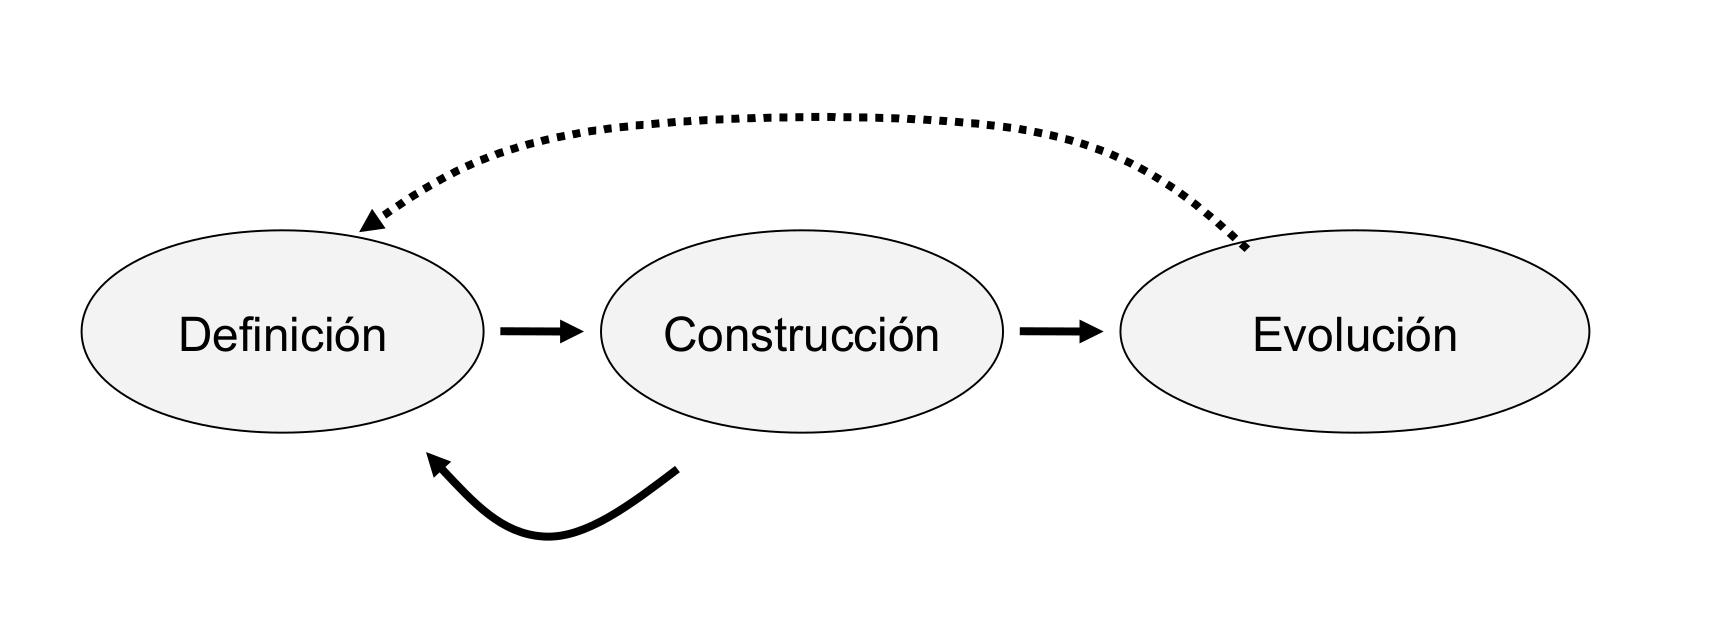
\includegraphics[scale=0.2]{proceso_produccion.png}
\caption{Etapas del proceso de producción del software.}
\end{figure}

\begin{figure}[H]
	\centering
	\begin{subfigure}[b]{0.4\textwidth}
	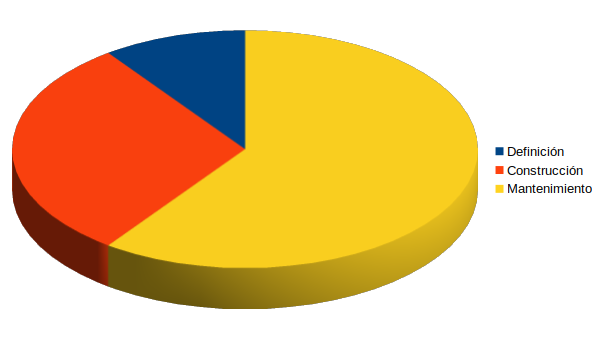
\includegraphics[width=\textwidth]{esfuerzo_etapas.png}
	\caption{Esfuerzo invertido en las distintas etapas.}
	\end{subfigure}
	\qquad
	\begin{subfigure}[b]{0.4\textwidth}
	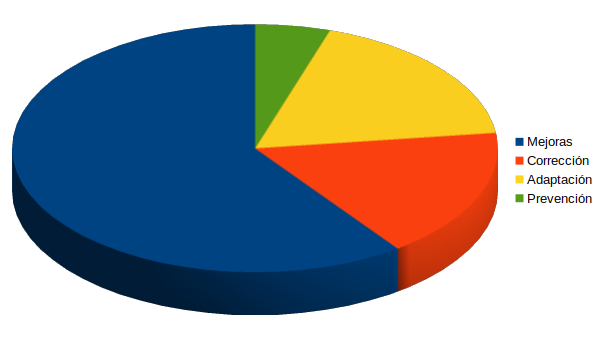
\includegraphics[width=\textwidth]{esfuerzo_mantenimiento.png}
	\caption{Esfuerzo invertido en las distintas etapas del mantenimiento.}
	\end{subfigure}
	\caption{Comparativa de esfuerzos.}
\end{figure}


\newpage

\subsubsection{Problemas en el desarrollo}

\begin{enumerate}
	\item \textbf{Comunicación} entre personas.
		\begin{figure}[H]
		\centering
		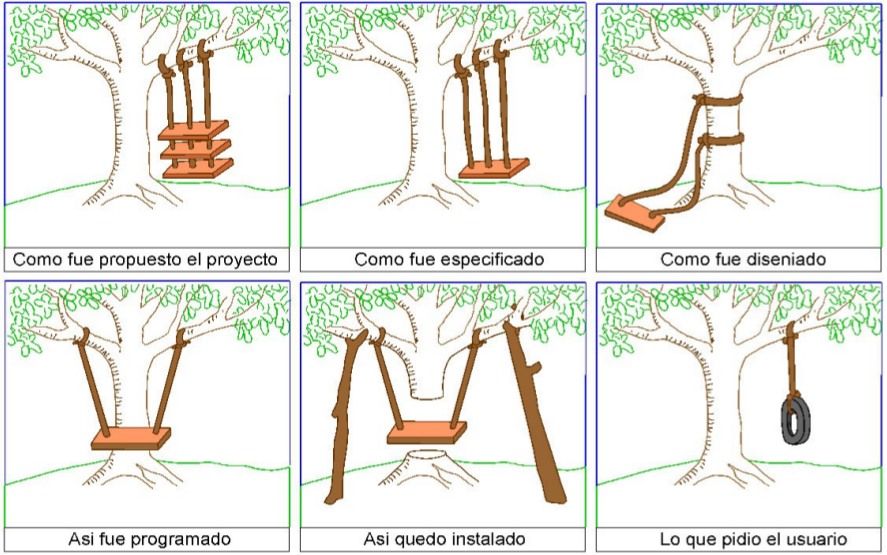
\includegraphics[scale=0.5]{problema_comunicacion.png}
		\caption{Problemas en la comunicación.}
		\end{figure}
	\item Incumplimiento de la \textbf{planificación}.
	\item Incorporación de \textbf{cambios} en etapas avanzadas.
		\begin{figure}[H]
		\centering
		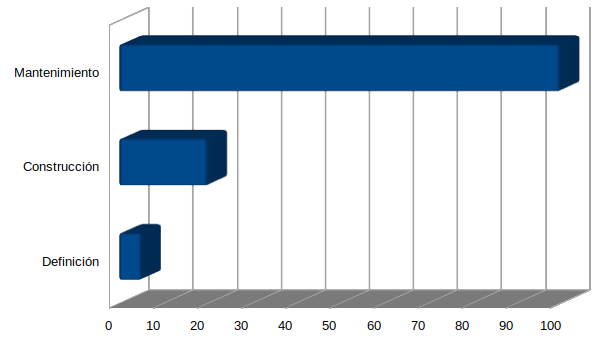
\includegraphics[scale=0.8]{impacto_cambio.png}
		\caption{Impacto del cambio en las distintas etapas.}
		\end{figure}
\end{enumerate}

\paragraph{Desastres ocasionados por sistemas software}
La mayoría de ellos tienen como causa pruebas deficientes, mala documentación, diseños pobres o inexistentes, mal estudio del problema, etc.

\subsection{Concepto de Ingeniería del Software}

La \emph{Ingeniería del Software} surgió por varias necesidades:
\begin{itemize}
	\item Mal funcionamiento (calidad).
	\item Mantenimiento del software existente.
	\item Demanda creciente del nuevo software.
	\item Adaptación a las nuevas tecnologías.
	\item Incremento de la complejidad.
\end{itemize}

\subsubsection{Definiciones de la Ingeniería del Software}

\begin{enumerate}
	\item Establecimiento de los principios y métodos de la ingeniería a fin de obtener software de modo rentable que sea fiable y trabaje en máquinas reales.
	\item Aplicación práctica del conocimiento científico en el diseño y construcción de programas de computadora y la documentación asociada y requerida para el desarrollo, operación y mantenimiento del programa.
	\item Estudio de los principios y métodos para el desarrollo y mantenimiento de sistemas software.
	\item Aplicación de un enfoque sistémico, disciplinado y cuantificable al desarrollo, operación y mantenimiento del software; es decir, aplicación de la ingeniería al software.
	\item Conjunto de teorías, métodos e instrumentos (tecnológicos y organizativos) que permitan construir sistemas software con las características de calidad deseadas.
	\item Disciplina de ingeniería que se interesa por todos los aspectos de la producción de software, desde las primerasa etapas de la especificación hasta el mantenimiento del sistema después de su puesta en operación.
\end{enumerate}

\subsubsection{Terminología usada en Ingeniería del Software}

\begin{itemize}
	\item \textbf{Sistema}. Conjunto de elementos relacionados entre sí y con el medio, que forman una unidad o un todo organizativo.
	\item \textbf{Sistema basado en computadora}. Conjunto o disposición de elementos organizados para cumplir una meta predefinida al procesar información.
		\begin{figure}[H]
		\centering
		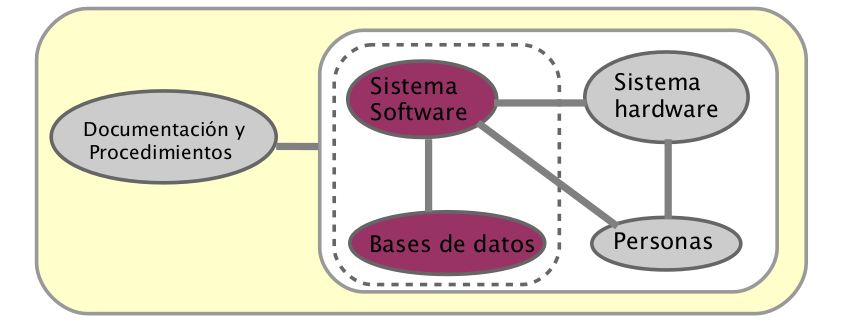
\includegraphics[scale=0.35]{sist_basado_comp.png}
		\caption{Sistema basado en computadora.}
		\end{figure}
	\item \textbf{Sistema Software}. Conjunto de piezas o elementos software relacionados entre sí y organizados en subsistemas.
		\begin{figure}[H]
		\centering
		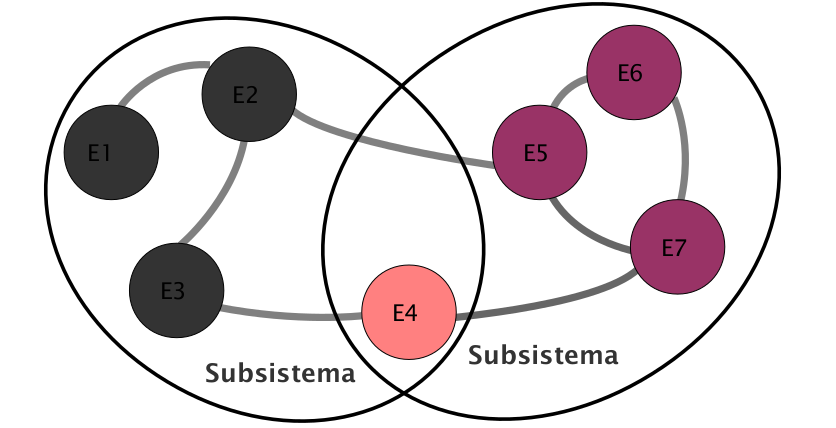
\includegraphics[scale=0.35]{sist_software.png}
		\caption{Sistema Software.}
		\end{figure}
	\item \textbf{Modelo}. Representación de un problema en un determinado lenguaje. De un mismo problema se pueden construir muchos modelos.
		\begin{figure}[H]
		\centering
		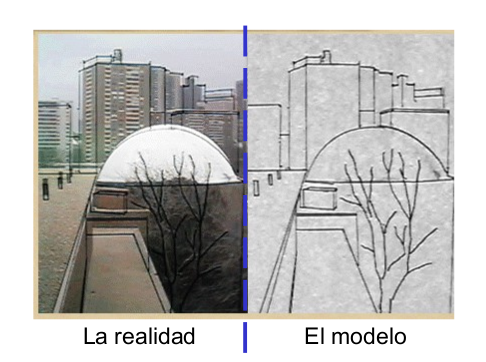
\includegraphics[scale=0.65]{modelo.png}
		\caption{Modelo.}
		\end{figure}
	\item \textbf{Principio}. Elementos que son adquiridos mediante el conocimiento. Determinan las características que debe poseer un modelo para ser una representación adecuada de un sistema.
	\item \textbf{Herramienta}. Instrumentos que permiten la representación de modelos.
	\item \textbf{Técnica}. Modo de utilización de las herramientas.
	\item \textbf{Heurísticas}. Conjunto de reglas empíricas que al ser aplicadas producen modelos que se adecuan a los principios. Ejemplo: \textit{No usar materiales flexibles para representar la maqueta de un edificio}.
	\item \textbf{Proceso}. Estructura que debe establecerse para la obtención eficaz de un producto de Ingeniería.
	\item \textbf{Método}. Proporciona la experiencia técnica para elaborar el producto software. Se basa en principios fundamentales e incluye actividades de modelado.
	
\end{itemize}

\subsection{Proceso de desarrollo del software}

\subsubsection{Concepto de proceso de desarrollo}

\begin{itemize}
	\item \textbf{Proceso de desarrollo del software}. Conjunto de \emph{actividades, acciones y tareas} que se realizan cuando va a crearse un producto o sistema software.
	\item \textbf{Actividad}. Busca el logro de objetivos amplios e independientes del tipo de aplicación a desarrollar y su complejidad.
	\item \textbf{Acción}. Conjunto de tareas que elaboran un producto importante como resultado.
	\item \textbf{Tarea}. Objetivo pequeño y bien definido que produce un resultado tangible.
\end{itemize}

Las actividades que se realizan pueden ser de varios tipos:

\begin{enumerate}
	\item \textbf{Estructurales}. Se dedican a obtener el producto:
		\begin{enumerate}
			\item \textbf{Comunicación}. Colaboración con el cliente para entender los objetivos y requisitos del proyecto.
			\item \textbf{Planificación}. Definición del plan de proyecto en el que se describen los riesgos probables, recursos adquiridos y productos obtenidos a la vez que se programan las actividades, acciones y tareas.
			\item \textbf{Modelado}. Representación mediante modelos del sistema porpuesto junto con la solución o soluciones apropiadas.
			\item \textbf{Construcción}. Generación de código y su prueba.
			\item \textbf{Despliegue}. Entrega al consumidor y evaluación por parte de éste, lo que sirve como retroalimentación para el equipo de desarrollo.
		\end{enumerate}

	\item \textbf{Sombrilla}. Se aplican a lo largo de todo el proceso. Se dedican a:
		\begin{enumerate}
			\item Seguimiento y control del proyecto.
			\item Administración del riesgo.
			\item Aseguramiento de la calidad.
			\item Revisiones técnicas.
			\item Mediciones de parámetros del proceso.
			\item Administración de la configuración.
			\item Administración de la reutilización.
			\item Preparación y producción del producto de trabajo.
		\end{enumerate}
	
\end{enumerate}

\subsubsection{Modelo general de proceso}
\begin{itemize}
	\item \textbf{Estructura del proceso}. Cada una de las actividades, acciones y tareas se encuadran dentro de una estructura que define su relación con el proceso y entre ellas.
		\begin{figure}[H]
		\centering
		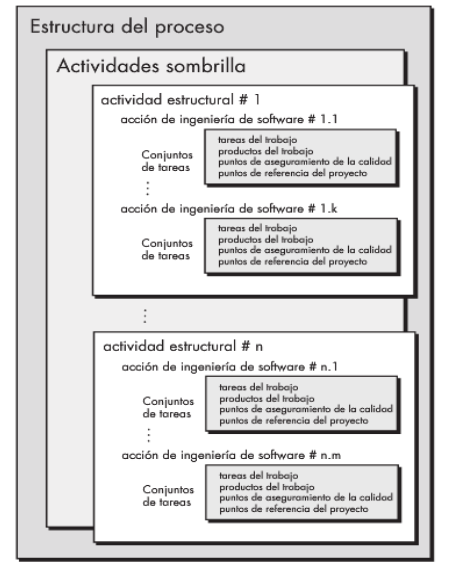
\includegraphics[scale=0.5]{estructura_proceso.png}
		\caption{Estructura del proceso.}
		\end{figure}	
	\item \textbf{Flujo del proceso}. Describe la forma en la que se organizan las actividades estructurales, acciones y tareas en los procesos con respecto a la secuencia y el tiempo.
		\begin{figure}[H]
			\centering
			\begin{subfigure}[H]{0.5\textwidth}
			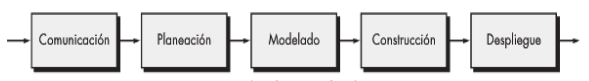
\includegraphics[width=\textwidth]{proceso_lineal.png}
			\caption{Flujo de proceso lineal.}
			\end{subfigure}
			\vskip 10pt
			\begin{subfigure}[H]{0.5\textwidth}
			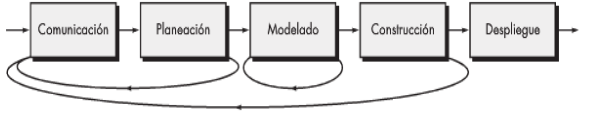
\includegraphics[width=\textwidth]{proceso_iterativo.png}
			\caption{Flujo de proceso iterativo.}
			\end{subfigure}
			
			\begin{subfigure}[H]{0.5\textwidth}
			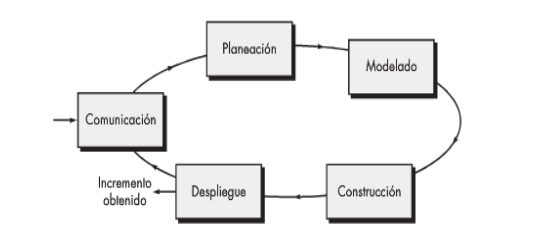
\includegraphics[width=\textwidth]{proceso_evolutivo.png}
			\caption{Flujo de proceso evolutivo.}
			\end{subfigure}
			\caption{Tipos de flujos de proceso.}
		\end{figure}
	\item \textbf{Acciones y tareas de las actividades estructurales}.
		\begin{enumerate}
			\item \textbf{Obtención de requisitos}. Obtención de información respecto a la acción que debe realizar el software.
			\item \textbf{Estimación y planificación del proyecto}. Estimar el tiempo y los costes del desarrollo del software.
			\item \textbf{Análisis de requisitos}. Documento en el que se especifica lo que debe hacer el sistema software.
			\item \textbf{Diseño}. Búsqueda de la solución. Descripción de los componentes, sus relaciones y funciones que le dan solución al problema.
			\item \textbf{Implementación}. Traducción del diseño a un lenguaje de programación entendible por una máquina.
			\item \textbf{Prueba del software}. Revisión y validación del código que se va desarrollando.
			\item \textbf{Evaluación y aceptación}. Evaluación del producto y aceptación por parte de los interesados en él.
			\item \textbf{Entrega y asistencia}. Sistema pasa a operar y se ofrece asistencia para su correcto funcionamiento.
		\end{enumerate}
\end{itemize}

\subsubsection{Tipos de modelos de proceso}

\begin{itemize}
	\item \textbf{Modelo en cascada}. Presenta una estructura secuencial y un flujo lineal. Sin embargo, los proyectos no suelen adecuarse a este modelo, es difícil expresar los requisitos a través de él al principio del proyecto y ofrece poca comunicación con el cliente, ya que hasta el final no hay un ejecutable que se pueda evaluar.
		\begin{figure}[H]
			\centering
			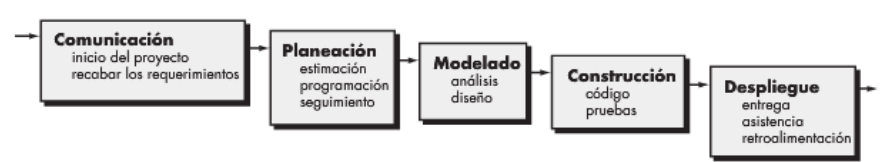
\includegraphics[scale=0.5]{modelo_cascada.png}
			\caption{Modelo en cascada.}
		\end{figure}
	\newpage
	\item \textbf{Modelo incremental}. Su estructura es secuencial mientras  que el flujo de proceso es lineal y paralelo entre incrementos.
			\begin{figure}[H]
			\centering
			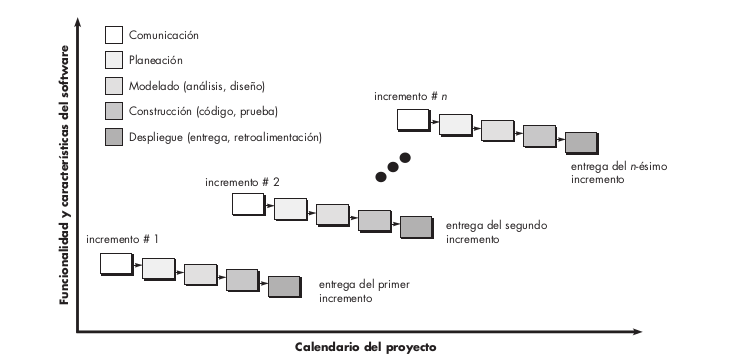
\includegraphics[scale=0.5]{modelo_incremental.png}
			\caption{Modelo incremental.}
		\end{figure}
	\item \textbf{Modelo evolutivo}. Es también iterativo. Nace como solución a varios factores, como un tiempo de entrega muy limitado o la necesidad de facilitar la incorporación de cambios. En cada iteración del proceso se obtiene un producto terminado y operativo. Sus características generales son:
	\begin{enumerate}
		\item Afrontan los riesgos altos (técnicos, de requisitos, etc.) tan pronto como sea posible.
		\item Retroalimentación temprana por parte del cliente.
		\item Manejo de la complejidad (pasos cortos y sencillos).
		\item El conocimiento adquirido durante una iteración de la evolución se puede usar en el resto de iteraciones.
		\item Involucra continuamente al usuario (evaluación, retroalimentación, afinamiento y refinamiento de requisitos, etc.).
	\end{enumerate}
	\newpage
	Hay dos tipos fundamentales de modelos evolutivos:
	\begin{enumerate}
		\item \textbf{Modelo de prototipos}. Un prototipo es una representación limitada de un producto que se utiliza para probar su diseño y comprender mejor el problema y sus posibles soluciones. Los prototipos pueden ser \emph{evolutivos} (productos finales) o \emph{desechables} (usados dentro de otros modelos de proceso).
		\begin{figure}[H]
		\centering
		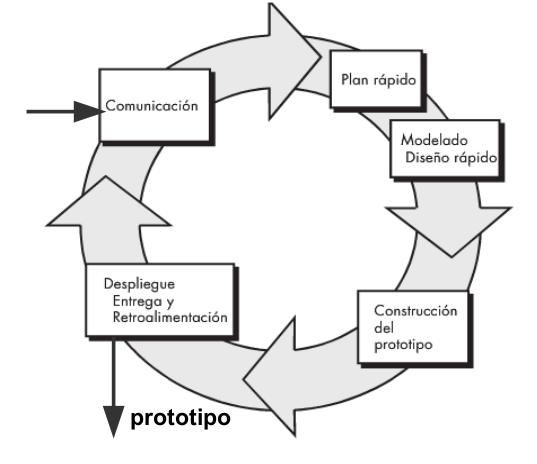
\includegraphics[scale=0.5]{modelo_prototipos.png}
		\caption{Modelo de prototipos}
		\end{figure}
	\end{enumerate}
	Este modelo se utiliza para:
	\begin{enumerate}
		\item Facilitar la obtención y validación de requisitos (\emph{desechable}).
		\item Estudios de viabilidad (\emph{desechable}).
		\item Propuestas de diseños alternativos (\emph{desechable}).
		\item En casos muy concretos como producto final (\emph{evolutivo}). 
	\end{enumerate}
	Presentan todas las características de los modelos evolutivos, aunque se les añaden algunos inconvenientes:
	\begin{itemize}
		\item Crear falsas expectativas por parte del cliente (\emph{desechable}).
		\item Puede que el prototipo \emph{desechable} se elabore con una metodología ineficiente y ésta se mantenga en el producto final.
	\end{itemize}
	\item \textbf{Modelo en espiral de Boehm}. Además de las características de los procesos iterativos, incluye otras más:
	\begin{enumerate}
		\item Se centra en el análisis de riesgo, construyendo prototipos para su estudio.
		\item La espiral puede continuar una vez que se entregue el momento para llevar a cabo el mantenimiento.
		\item Es adecuado para el desarrollo de sistemas a gran escala.
	\end{enumerate}
	Sus principales inconvenientes son que no es controlable y que requiere un equipo de desarrollo con gran experiencia en análisis de riesgo.
	\begin{figure}[H]
		\centering
		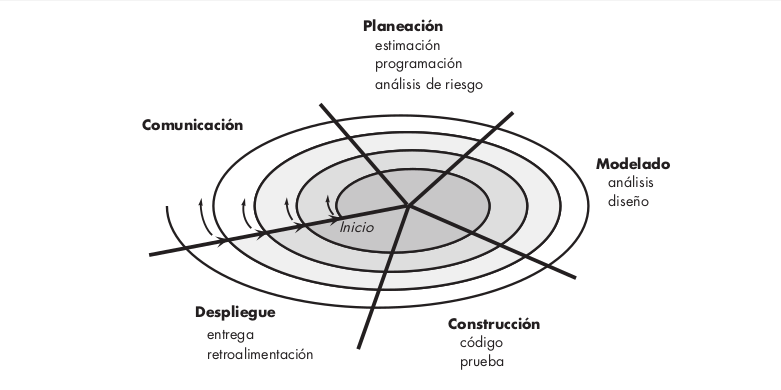
\includegraphics[scale=0.5]{modelo_espiral.png}
		\caption{Modelo en espiral de Boehm}
	\end{figure}
\end{itemize}

\subsubsection{Proceso unificado}
Es un modelo de proceso evolutivo y compuesto por cuatro fases:
\begin{itemize}
	\item Inicio o concepción.
	\item Elaboración.
	\item Construcción.
	\item Transición.
\end{itemize}
Estas etapas se reparten entre las actividades estructurales como podemos ver en el diagrama:

\begin{figure}[H]
			\centering
			\begin{subfigure}[b]{0.4\textwidth}
			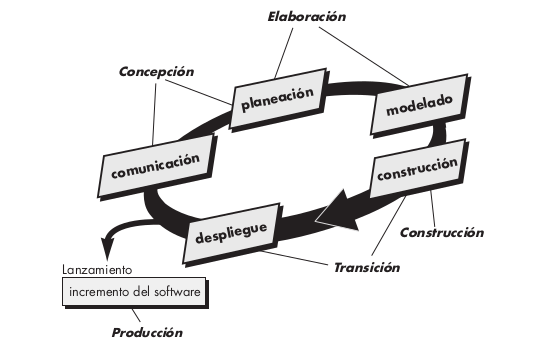
\includegraphics[width=\textwidth]{proceso_unificado.png}
			\end{subfigure}
			\quad
			\begin{subfigure}[b]{0.5\textwidth}
			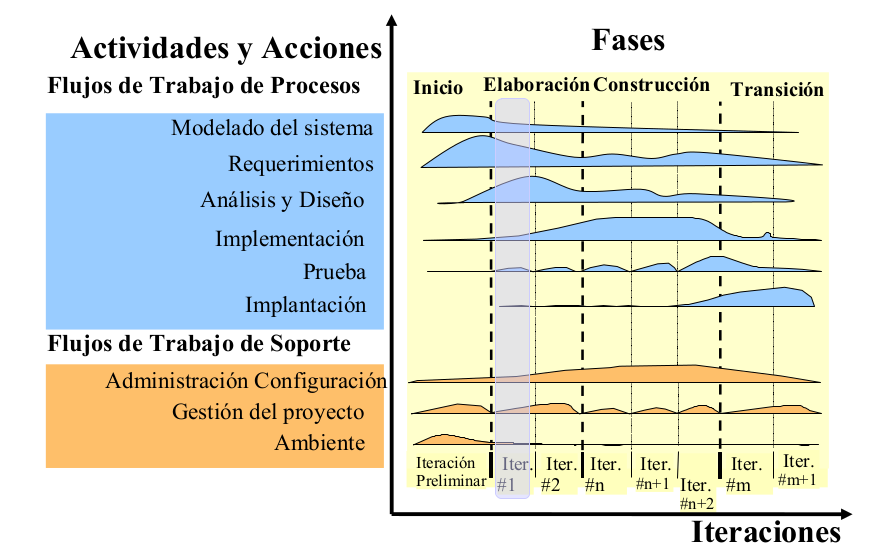
\includegraphics[width=\textwidth]{proceso_unificado_2.png}
			\end{subfigure}

			\caption{Proceso unificado.}
\end{figure}
\newpage
Además de las características de los modelos de proceso evolutivos, el proceso unificado incorpora las siguientes:
\begin{enumerate}
	\item Es un modelo de proceso adaptable a la complejidad y al tipo de sistema.
	\item Está centrado en la arquitectura, mostrando y decidiendo los distintos aspectos arquitectónicos de un sistema software en etapas tempranas. De esta forma pueden servir de base a las posteriores.
	\item Está dirigido por casos de uso, desarrollándose uno o varios en cada iteración. En iteraciones tempranas los casos de uso determinarán la arquitectura.
\end{enumerate}
\paragraph{Acciones y tareas en cada fase}
\begin{itemize}
	\item \textbf{Inicio}. Agrupa actividades tanto de comunicación del cliente como de planificación. Se propone una arquitectura aproximada para el sistema y se estudian numerosos factores (viabilidad, alcance, riesgos, etc.).
	\item \textbf{Elaboración}. Incluye actividades de comunicación y modelado de la arquitectura básica sobre la que se asentará la fase de construcción.
	\item \textbf{Construcción}. Se completan los modelos de requisitos y se implementan los elementos necesarios para completar el sistema. Según se van terminando los elementos, son probados e integrados al producto final. También se realizan pruebas de aceptación por parte del usuario.
	\item \textbf{Transición}. Consiste en asegurarse de que el sistema cumple con los requisitos especificados (mediante pruebas por parte de los usuarios). Además, se genera el material necesario para lanzar el producto al mercado.
\end{itemize}

\begin{figure}[H]
	\centering
	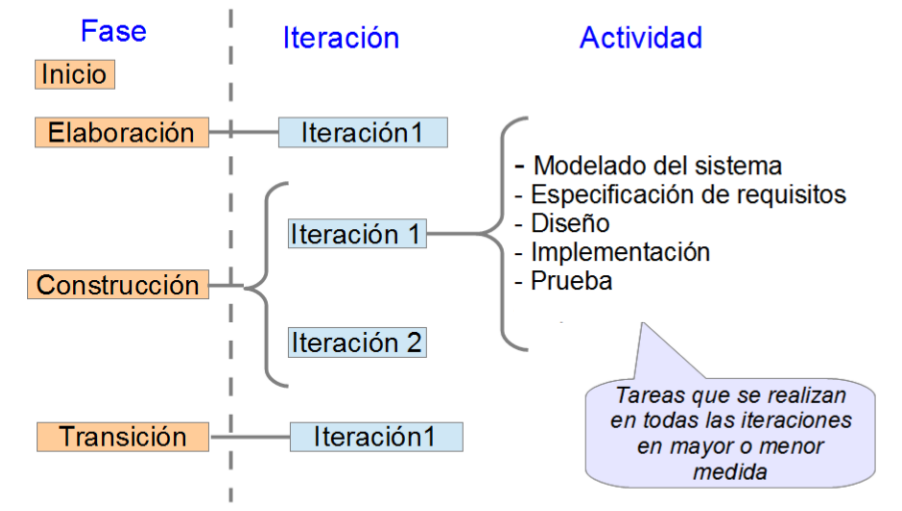
\includegraphics[scale=0.45]{proceso_unificado_ej.png}
	\caption{Ejemplo de Proceso Unificado}
\end{figure}

\subsubsection{Desarrollo Ágil}
En 2001, diecisiete expertos se preguntaron por qué muchos proyectos generaban menos valor del esperado, no se terminaban a tiempo, tenían problemas de calidad serios, etc. Tras ésto, elaboraron el \emph{Manifiesto el Desarrollo Ágil de Software} con el que intentaban dar solución a estos problemas.
\paragraph{Características del Desarrollo Ágil}
\begin{enumerate}
	\item Es un proceso iterativo e incremental, por lo que es evolutivo.
	\item Requiere entregas frecuentes y trabajo en equipo.
	\item Establece autonomía en el equipo de desarrollo.
	\item Exige revisiones y reuniones retrospectivas frecuentes.
\end{enumerate}
Sus beneficios son que se mejora la productividad y que se manejan mejor los riesgos.\\
Consta de varias técnicas:
\begin{itemize}
	\item Scrum
	\item XP (\emph{Extreme Programming})
	\item Programación en parejas.
	\item TDD (\emph{Test Driven Development})
\end{itemize}

\newpage

 
\section{Tema 2. Ingeniería de Requisitos}

\subsection{Introducción}

En 1995 se realizó el informe \emph{CHAOS} sobre los resultados que se obtuvieron en diversos proyectos software:
\begin{figure}[H]
\centering
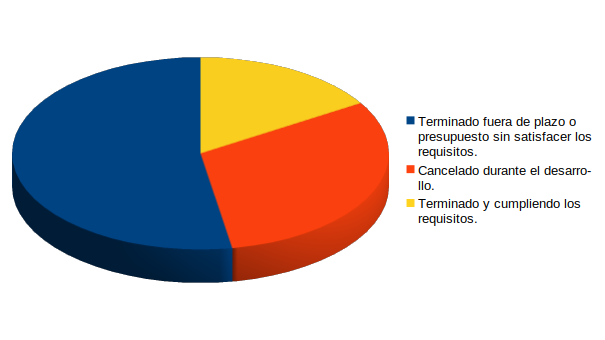
\includegraphics[scale=0.5]{informe_chaos.png}
\caption{Resultados del informe \emph{CHAOS}.}
\end{figure}

Los principales factores de fracaso son:

\begin{enumerate}
	\item Falta de información por parte de los usuarios.
	\item Especificación de requisitos incompleta.
	\item Continuos cambios de los requisitos.
	\item Pobres habilidades técnicas en la especificación de requisitos.
\end{enumerate}

La \textbf{Ingeniería de Requisitos} cubre las tareas y proporciona los mecanismos adecuados para:
\begin{itemize}
	\item Entender y analizar las necesidades del cliente.
	\item Evaluar la viabilidad de las necesidades.
	\item Negociar una solución razonable.
	\item Especificar la solución sin ambigüedades, confeccionando un documento que describa la solución acordada.
	\item Validar y analizar la especificación reflejada en el documento de especificación de requisitos, obteniendo el \emph{modelo de análisis}.
	\item Administrar y desarrollar los requisitos a lo largo del proceso de desarrollo.
\end{itemize}

El proceso de construcción de una \emph{especificación de requisitos} es iterativo. En él, partimos de las especificaciones iniciales imcompletas, poco claras y ambiguas y llegamos a especificaciones finales \textbf{completas, claras, documentadas y validadas}.

\subsubsection{Concepto de requisito y tipos}
Un requisito se puede definir de varias formas:
\begin{itemize}
	\item Condición o capacidad que debe tener un producto software para resolver la necesidad expresada por un usuario.
	\item Representación en forma de documento de una capacidad o condición que debe tener un producto software.
	\item Característica de un productor software que es condición para su aceptación por parte del cliente.
	\item Propiedad o restricción determinada con precisión que un producto software debe satisfacer.
\end{itemize}

\paragraph{Tipos de requisito}
Los requisitos se pueden clasificar según varios factores:
\begin{figure}[H]
\centering
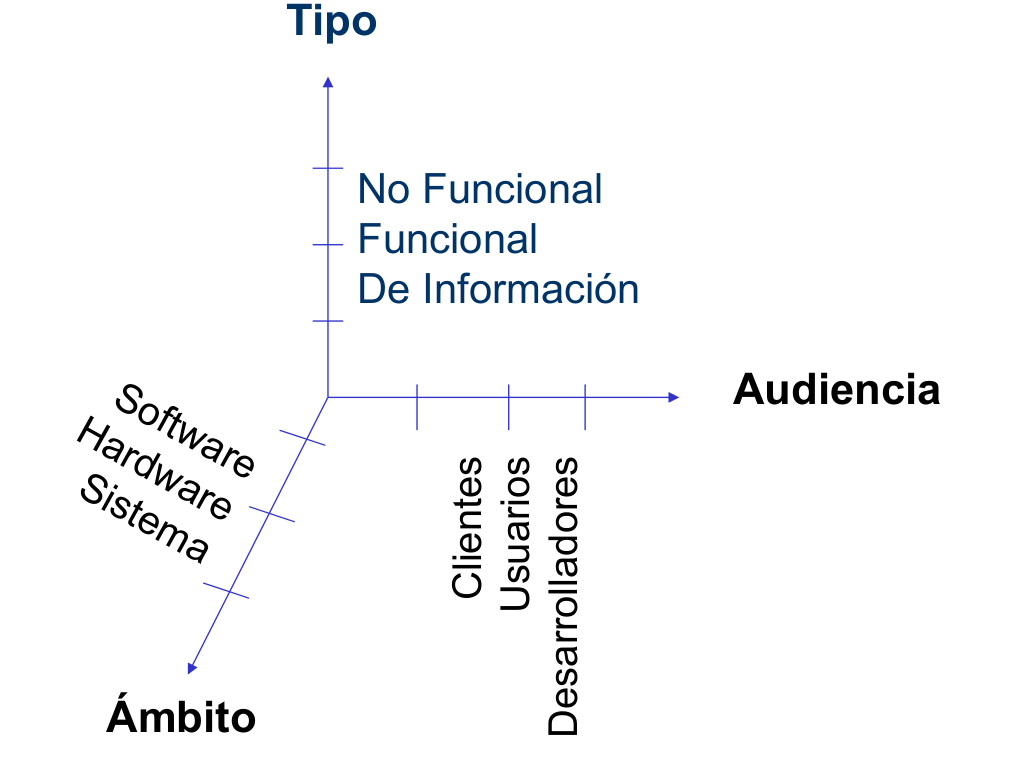
\includegraphics[scale=0.25]{tipos_requisito.png}
\caption{Tipos de requisito.}
\end{figure}

\begin{enumerate}
	\item \textbf{Funcionales}. Describen la interacción entre el sistema y su entorno, proporcionando servicios que proveerá el sistema o indicando la forma en la que reaccionará ante determinados estímulos.
	\item \textbf{No funcionales o atributo de calidad}. Describen cualidades o restricciones del sistema que no se relacionan de forma directa con el comportamiento funcional del mismo.
	\begin{itemize}
		\item Restringen los tipos de soluciones que podemos tomar y suelen restringir el diseño que se realice.
		\item No describen funciones, sino propiedades (rendimiento, fiabilidad, seguridad, etc.).
		\item Son los que garantizan la calidad del software.
		\item Pueden ser requisitos de producto, de organización o externos.
		\item Son difíciles de determinar.
	\end{itemize}
	\item \textbf{De información}. Describen necesidades de almacenamiento de información en el sistema.
\end{enumerate}

\subparagraph{Clasificación FURPS+}

\begin{itemize}
	\item Funcionalidad (\textbf{F}uncionality): requisito funcional.
	\item Facilidad de uso (\textbf{U}sability): factores humanos, ayuda, documentación.
	\item Rendimiento (\textbf{P}erformance): tiempos de respuesta, productividad, etc.
	\item Soporte (\textbf{S}upportability): adaptabilidad, facilidad de mantenimiento, etc.
	\item Pseudorrequisitos o restricciones de diseño (\textbf{+}):
		\begin{itemize}
			\item \textbf{Implementación}: limitación de recursos, lenguajes, etc.
			\item \textbf{Interfaz}: restricciones impuestas para la interacción con sistemas externos.
			\item \textbf{Operación}: gestión del sistema en su puesta en marcha y a nivel operacional.
			\item \textbf{Empaquetamiento}: formas de distribución, restricciones de instalación, etc.
			\item \textbf{Legales}: licencias, derechos de autor, etc.
		\end{itemize}
\end{itemize}

\paragraph{Ejemplos de requisitos}

\begin{itemize}
	\item El sistema debe validar la tarjeta en menos de tres segundos.
	\item El sistema debe contar el número de palabras procesadas.
	\item El sistema se diseñará para un terminal CRT monocromo.
	\item Los usuarios del sistema serán en su mayoría novatos.
	\item Deben producirse informes útiles
\end{itemize}



\subsubsection{Propiedades de los requisitos}

Para que los requisitos sean de calidad deben satisfacer las siguientes propiedades:

\begin{itemize}
	\item \textbf{Completos}. Todos los aspectos del sistema deben estar representados en el modelo de requisitos.
	\item \textbf{Consistentes}. Los requisitos no deben contradecirse entre sí.
	\item \textbf{No ambiguos}. No se deben poder interpretar los requisitos de varias formas distintas.
	\item \textbf{Correctos}. Deben representar exactamente el sistema que el cliente necesita y que el desarrollador construirá.
	\item \textbf{Realistas}. Los requisitos se deben poder implementar con la tecnología y presupuesto disponible.
	\item \textbf{Verificables}. Se deben poder diseñar pruebas para demostrar que el sistema satisface los requisitos.
	\item \textbf{Trazables}. Cada requisito debe poder rastrearse a través del desarrollo del software hasta su conveniente funcionalidad del sistema.
\end{itemize}


\subsubsection{Tareas de la Ingeniería de Requisitos}

\begin{enumerate}
	\item \textbf{Estudio de viabilidad}. ¿Es conveniente desarrollar el sistema?
		\begin{itemize}
			\item ¿Soluciona el software los problemas existentes?
			\item ¿Se puede desarrollar con la tecnología actual?
			\item ¿Se puede desarrollar con las restricciones de costo y tiempo?
			\item ¿Puede integrarse con otros existentes en la organización?
		\end{itemize}
		Este paso finaliza con la obtención del \emph{informe de viabilidad}.
	\item \textbf{Obtención de requisitos}. Trabajo con clientes y usuarios para:
		\begin{itemize}
			\item Estudiar el funcionamiento del sistema.
			\item Descubrir las necesidades reales.
			\item Consensuar los requisitos entre las distintas partes.
		\end{itemize}
		Es un proceso difícil apoyado por diversas técnicas, como entrevistas, prototipados, casos de uso, etc. 
		\item \textbf{Análisis de requisitos}. Es la actividad más importante. Sus objetivos son:
			\begin{itemize}
				\item Detectar conflictos entre requisitos.
				\item Profundizar en el conocimiento del sistema.
				\item Establecer las bases para el diseño.
				\item Construir modelos abstractos.
			\end{itemize}
			\begin{figure}[H]
				\centering
				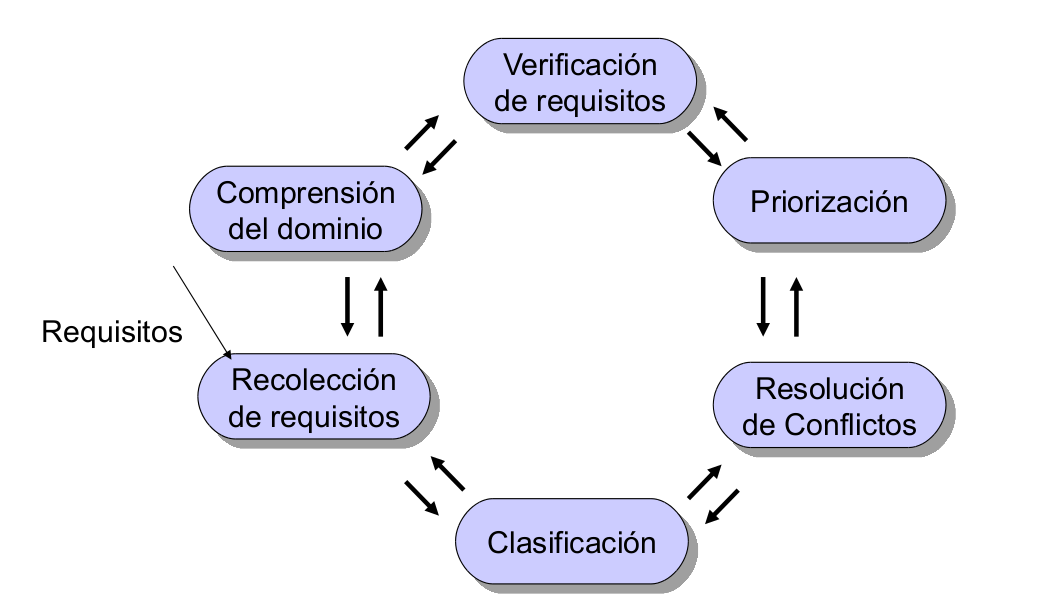
\includegraphics[scale=0.25]{actividades_analisis_requisitos.png}
				\caption{Actividades en el análisis de requisitos.}
			\end{figure}
		\item \textbf{Especificación de requisitos}. Consiste en representar los requisitos en base al modelo creado en el análisis.
		\newpage
		\item \textbf{Revisión de requisitos}
			\begin{itemize}
				\item \textbf{Validación}$^1$. Consiste en ver que los requisitos reflejan el problema a solucionar.
				\item \textbf{Verificación}$^2$. Consiste en comprobar que la representación sea correcta.
			\end{itemize}
			Es un proceso continuo durante todo el desarrollo.
			\begin{figure}[H]
				\centering
				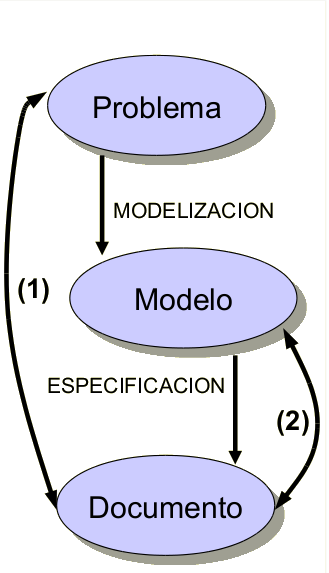
\includegraphics[scale=0.3]{revision_requisitos.png}
				\caption{Revisión de requisitos.}
			\end{figure}
\end{enumerate}

En cada fase obtenemos una serie de productos: 

\begin{itemize}
	\item En la \textbf{obtención de requisitos}.
		\begin{enumerate}
			\item Documentos de entrevistas.
			\item Lista estructurada de requisitos.
			\item Diagramas de casos de uso, plantillas de casos de uso y diagramas de actividad.
		\end{enumerate}
	\item En la \textbf{especificación de requisitos}.
		\begin{itemize}
			\item Modelo arquitectónico (subsistemas) $\rightarrow$ Diagrama de paquetes.
			\item Modelo estático (conceptual) $\rightarrow$ Diagrama de clases.
			\item Modelo dinámico (funcional) $\rightarrow$ Diagrama de secuencia del sistema y contratos.
		\end{itemize}
\end{itemize}

\subsubsection{Roles}

En la ingeniería de requisitos podemos distinguir varios roles: 

\begin{itemize}
	\item Stakeholder (personas que tienen relación con el sistema).
	\item Ingeniero de requisitos.
	\item Analista de sistemas.
	\item Arquitecto de software (diseño).
	\item Documentalista.
	\item Diseñador de Interfaces de Usuario.
	\item Gestor de proyecto,
	\item Revisor.
\end{itemize}

\subsubsection{Problemas de la Ingeniería de Requisitos}

Podemos agruparlos en 3 áreas:

\begin{itemize}
	\item Dificultades para \textbf{obtener información}.
	\item Manejo de la \textbf{complejidad del problema}.
	\item Dificultades para la \textbf{integración de los cambios}.
\end{itemize}

Pueden estar causados por:

\begin{itemize}
	\item Pobre comunicación
	\item Uso de técnicas inapropiadas.
	\item Tendencias a acortar el análisis.
	\item No considerar alternativas.
\end{itemize}

\subsection{Obtención de Requisitos}

\subsubsection{Proceso de obtención de requisitos}

La obtención de requisitos es la fase inicial de la ingeniería de requisitos. Necesitamos obtener:
\begin{itemize}
	\item Necesidades y características del sistema.
	\item Informe del alcance del sistema o producto.
	\item Lista de participantes.
	\item Descripción del entorno técnico.
	\item Lista de los requisitos agrupados por su funcionalidad junto a las correspondientes restricciones que se aplicarán a cada uno.
\end{itemize}
\newpage
Las tareas que se deben realizar son las siguientes: 

\begin{enumerate}
	\item Obtener información sobre el dominio del problema y el sistema actual.
		\begin{itemize}
			\item Conocer el vocabulario propio.
			\item Conocer las características principales del dominio.
			\item Recopilar información sobre el dominio (consultas con expertos, libros, etc.)
			\item Facilitar la comprensión de las necesidades del sistema.
			\item Favorecer la confianza del cliente.
		\end{itemize}
	Se ha de entregar la \emph{introducción al sistema} y el \emph{glosario de términos}.
	\item Preparar las reuniones de elicitación y negociación.
		\begin{itemize}
			\item Identificar a los implicados, realizando una descripción general de todos y del perfil de cada uno de ellos.
			\item Conocer las necesidades de los clientes y usuarios.
			\item Resolver los posibles conflictos
		\end{itemize}
	\item Identificar y revisar los objetivos del sistema. Si el sistema es muy complejo, podemos organizarlos mediante una jerarquía. De cada objetivo podemos describir:
		\begin{itemize}
			\item Su \textbf{importancia} (vital, importante o "quedaría bien").
			\item Su \textbf{urgencia} (inmediatamente, hay presión o puede esperar).
			\item Su \textbf{estado} durante el desarrollo (en construcción, pendiente de solución, validado, etc.)
			\item Su \textbf{estabilidad} (alta, media o baja).
		\end{itemize}
	\item Identificar y revisar los requisitos de información. De cada requisito podemos describir:
		\begin{itemize}
			\item Objetivos y otros requisitos asociados.
			\item Descripción del requisito.
			\item Contenido.
			\item Tiempo de vida (medio y máximo).
			\item Ocurrencias simultáneas (medio y máximo).
			\item Importancia, urgencia, etc.
		\end{itemize}
	\item Identificar y revisar los requisitos funcionales. Determinan lo que debe hacer el sistema. De cada requisito podemos describir:
		\begin{itemize}
			\item Objetivos y requisitos asociados.
			\item Secuencia de acciones.
			\item Frecuencia.
			\item Rendimiento.
			\item Importancia, urgencia, etc.
		\end{itemize}
	\item Identificar y revisar los requisitos no funcionales. Son las restricciones aplicables a los requisitos funcionales y de información. De cada requisito podemos definir:
		\begin{itemize}
			\item Descripción.
			\item Objetivos y requisitos asociados.
			\item Importancia, urgencia, etc.
		\end{itemize}
\end{enumerate}
Tras estos pasos se genera la \emph{lista estructurada de requisitos}.

\subsubsection{Técnicas de obtención}

\begin{itemize}
	\item Por \textbf{métodos tradicionales}: entrevistas, cuestionarios, análisis de protocolos, etc.
	\item Por \textbf{otros métodos}: técnicas orientadas a puntos de vista, escenarios y casos de uso, etc.
\end{itemize}

La información la poseen los implicados (\textit{stakeholders}). Un implicado puede ser todo aquel que se beneficia del sistema a construir directa o indirectamente o bien que posea información sobre su funcionamiento o desarrollo, como los responsables del mismo, el cliente, los responsables de la gestión, etc.
\subsubsection{Técnicas de entrevista}

Tienen el objetivo de obtener información sobre el sistema mediante el dialogo con los expertos en el dominio del problema. Las entrevistas pueden ser de varios tipos: estructuradas o no estructuradas y formales o informales.\\
Las fases de una entrevista son:
\begin{itemize}
	\item \textbf{Preparación}. Se estudia el dominio del problema, selecciona a los entrevistados y se planifican las entrevistas.
	\item \textbf{Realización}. Consta de:
		\begin{itemize}
			\item Apertura: presentación e informe sobre los objetivos de la entrevista.
			\item Desarrollo.
			\item Terminación: recapitulación de la información obtenida.

		\end{itemize}
	\item \textbf{Análisis}. Consiste en reorganizar la información, constatarla con otras fuentes , documentar la entrevista y enviar una copia al entrevistado.
\end{itemize}

Las principales limitaciones de una entrevista son que lo que los usuarios dicen no es siempre lo que hacen, la timidez y la interpretación de las preguntas. Sin embargo, aporta beneficios como la localización de las áreas en las que profundizar, la involucración de los clientes en el desarrollo o que es una técnica muy conocida y aceptada.

\subsubsection{Técnicas de análisis etnográfico}

Consiste en observar el contexto del sistema que afecta a los requisitos, es decir, observar la forma en la que las personas trabajan y no como el sistema las hace trabajar. 
\\
Hay dos tipos de observaciones: 
\begin{itemize}
	\item \textbf{Directa}. El observador está inmerso en el sistema.
	\item \textbf{Indirecta}. Se utilizan entornos de observación.
\end{itemize}

Se utilizan fundamentalmente para dos tipos de requisitos:
\begin{itemize}
	\item Los que derivan de la forma en la que trabajan realmente y no de cómo se han definido los procesos.
	\item Los que derivan de la cooperación y el conocimiento de las actividades de la gente.
\end{itemize}

No es un enfoque completo, sino que tiene que apoyarse en otras técnicas (entrevistas, prototipado, etc.)

\subsection{Modelado de Casos de Uso}

\subsubsection{Introducción}

El modelado de casos de uso es una técnica de la ingeniería de requisitos que permite:
\begin{itemize}
	\item Delimitar el sistema a estudiar.
	\item Determinar el contexto de uso del sistema.
	\item Describir el punto de vista de los usuarios del sistema.
\end{itemize}

El modelo de casos de uso se utiliza en distintas etapas del desarrollo para:
\begin{itemize}
	\item Obtener requisitos.
	\item Analizar y especificar requisitos.
	\item Como base para el proceso de diseño y su validación.
	\item Para guiar el diseño de la interfaz de usuario y facilitar la construcción de prototipos.
	\item Como punto de inicio de las ayudas en línea y el manual de usuario.
\end{itemize}

Elementos que componen el modelo de casos de uso:
\begin{itemize}
	\item Actores.
	\item Casos de uso.
	\item Relaciones entre:
		\begin{itemize}
			\item Actores.
			\item Actores y casos de uso.
			\item Casos de uso.
		\end{itemize}
\end{itemize}

Para representar y describir estos elementos se utilizan los \emph{diagramas de casos de uso de UML} y las \emph{plantillas estructuradas para actores y casos de uso}.

\subsubsection{Diagramas de Casos de Uso}

Es un diagrama UML que representa gráficamente todos los elementos que forman parte del modelo de casos de uso junto con la frontera del sistema.
\begin{figure}[H]
\centering
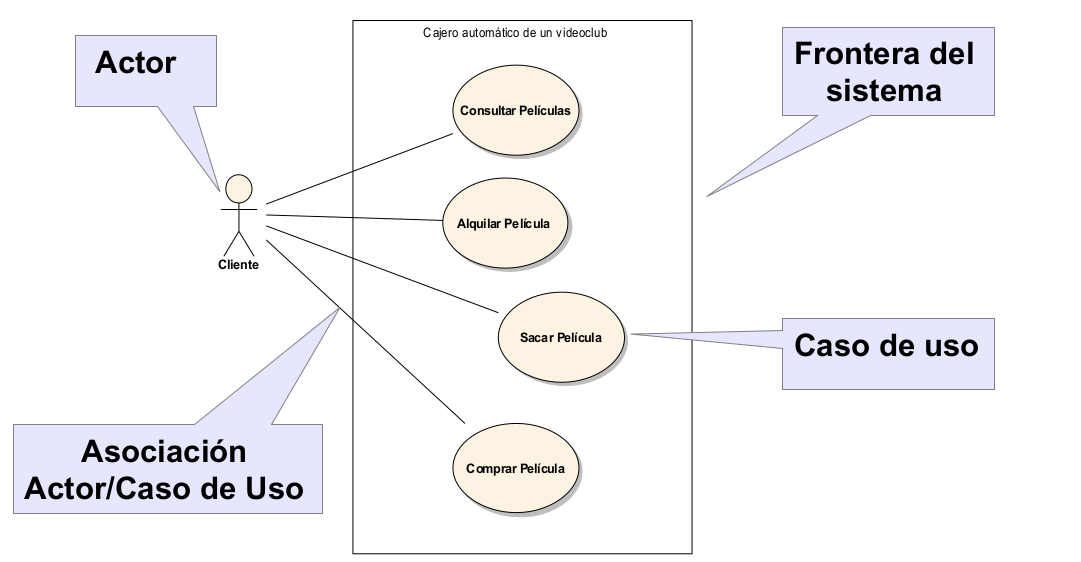
\includegraphics[scale=0.25]{diagramas_cu.png}
\caption{Diagrama de caso de uso}
\end{figure}

\subsubsection{Actor}

\paragraph{Definición}
Un actor es una abstracción de una \emph{entidad externa} al sistema que interactúa directamente con él.
\begin{itemize}
	\item Los actores especifican roles que adoptan las entidades externas cuando interactúan con el sistema.
	\item Una entidad puede desempeñar varios roles simultáneamente a lo largo del tiempo.
	\item Un rol puede ser desempeñado por varias entidades.
\end{itemize}

\begin{figure}[H]
	\centering
	\begin{subfigure}[b]{0.15\textwidth}
		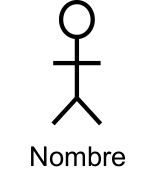
\includegraphics[width=\textwidth]{actor_1.png}
		\caption{}
	\end{subfigure}
	\quad
	\begin{subfigure}[b]{0.25\textwidth}
		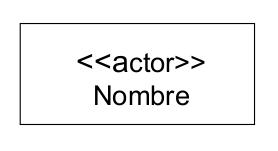
\includegraphics[width=\textwidth]{actor_2.png}
		\caption{}
	\end{subfigure}
	\caption{Representaciones de un actor en UML.}
\end{figure}

\paragraph{Características}
El nombre del rol debe ser breve y tener sentido desde la perspectiva de negocio. Es frecuente que coincidan con áreas de la empresa (vendedor, gestor de almacén) o distintos niveles de jerarquía (jefe, empleado, aprendiz).

\begin{figure}[H]
	\centering
	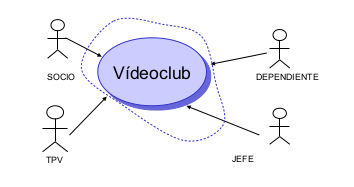
\includegraphics[scale=0.5]{actor_rol.png}
	\caption{Distintos roles para los actores.}
\end{figure}
	
\paragraph{Tipos de actores}

\begin{itemize}
	\item \textbf{Principales}. Además de interactuar con el caso de uso, son los que lo \emph{activan}.
	\item \textbf{Secundarios}. Interactúan con el caso de uso, pero no lo activan.
\end{itemize}

Los actores pueden ser:

\begin{itemize}
	\item \textbf{Personas} con el rol de usuario en el sistema.
	\item \textbf{Dispositivos de E/S} como sensores o medidores, simepre que sean independientes de la acción del usuario.
	\item \textbf{Sistemas informáticos externos} con los que se tiene que comunicar.
	\item \textbf{Temporizador} o reloj cuando se hace algo como respuesta a un evento de tiempo de tipo periódico o en un momento determinado, sin que haya un actor que lo active.
\end{itemize}

\begin{figure}[H]
	\centering
	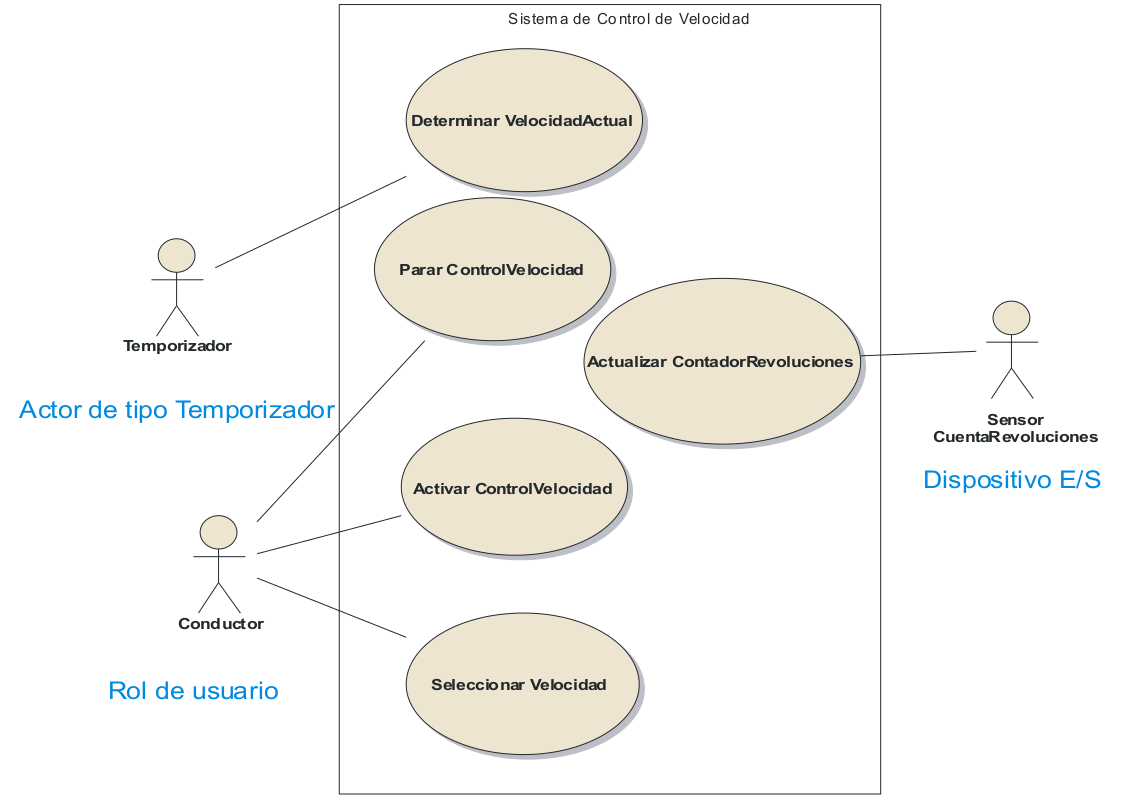
\includegraphics[scale=0.25]{actor_ej.png}
	\caption{Ejemplos de actores.}
\end{figure}

\paragraph{Identificación de actores}
Debemos responder a las siguientes preguntas:
\begin{itemize}
	\item ¿Quién y qué utiliza el sistema?
	\item ¿Qué roles desempeñan en la iteración?
	\item ¿Quién instala el sistema?
	\item ¿Quién o qué inicio y cierra el sistema?
	\item ¿Quién mantiene el sistema?
	\item ¿Qué otros sistemas interactúan con este sistema?
	\item ¿Quién o qué consigue y proporciona información al sistema?
\end{itemize}

\newpage

\paragraph{Relación entre actores\\\\}

\textbf{Generalización}. Expresa un comportamiento común entre actores, es decir, se relacionan de la misma forma con los mismos casos de uso.

\begin{figure}[H]
	\centering
	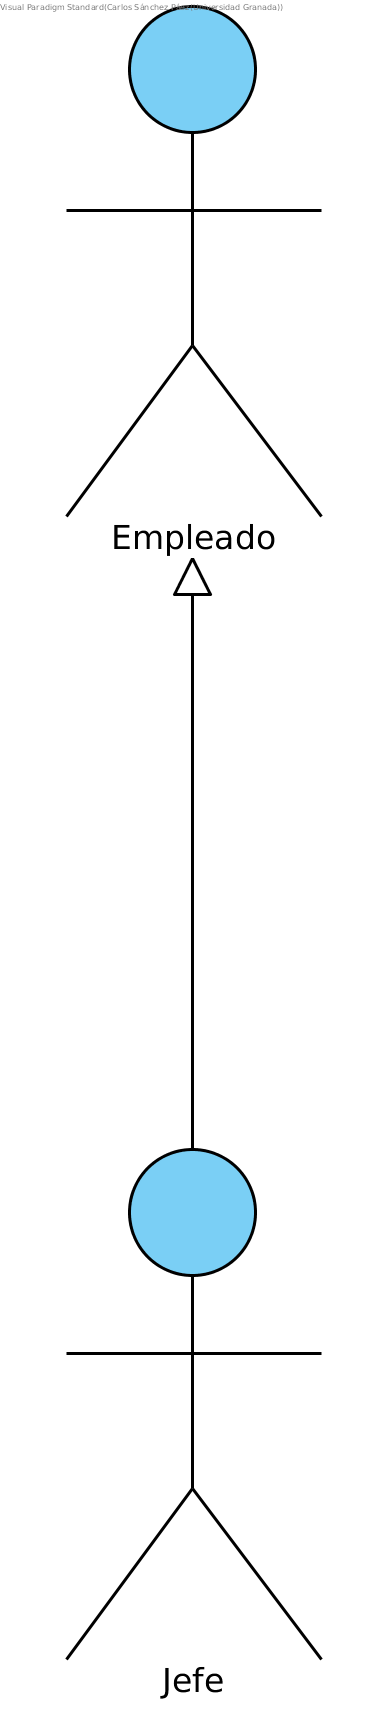
\includegraphics[scale=0.65]{actores_relacion.png}
	\caption{Relación entre actores.}
\end{figure}

Según esta relación:
\begin{itemize}
	\item Un empleado modela los aspectos comunes de cualquier tipo de empleado.
	\item Un jefe hereda los roles y la relaciones de los casos de uso del empleado, además de tener los suyos propios.
	\item Un actor jefe puede ser usado siempre en lugar de un actor empleado, ya que hereda sus roles y relaciones.
\end{itemize}


\subsubsection{Caso de Uso}

\paragraph{Definición}

Un caso de uso especifica la \emph{secuencia de acciones}, incluidas secuencias variantes y de error, que un sistema o subsistema puede realizar al interactuar con actores externos.

\begin{figure}[H]
	\centering
	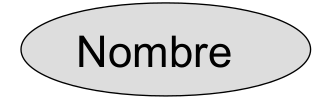
\includegraphics[scale=0.25]{cu_repr.png}
	\caption{Representación de un caso de uso.}
\end{figure}

El \emph{nombre} debe ser una frase verbal descriptiva y breve.\\
Dependiendo de su importancia, los casos de uso pueden ser:
\begin{itemize}
	\item \textbf{Primarios}. Procedimientos comunes más importantes (\emph{procesos de negocio}).
	\item \textbf{Secundarios}. Procesos de error o poco comunes (\emph{procesos internos, diseño}).
	\item \textbf{Opcionales}. Puede que no se implementen.
\end{itemize}

\paragraph{Características}

\begin{itemize}
	\item Son \emph{iniciados por un actor} que, junto con otros actores, intercambia datos o control con el sistema a a través de él.
	\item Son descritos desde el \emph{punto de vista de los actores} que interactúan con él.
	\item \emph{Describen} el proceso de \emph{alcance de un objetivo} de uno o varios actores.
	\item Tiene que tener una \emph{utilidad real y concreta} para algún actor.
	\item \emph{Acotan} una \emph{funcionalidad} del sistema.
	\item \emph{Describen} un fragmento de la \emph{funcionalidad} del sistema de principio a fin $\rightarrow$ tienen que acabar y dar algún resultado.
	\item Se documentan con \emph{texto informal}.
\end{itemize}

\begin{figure}[H]
\centering
\begin{tabular}{| m{3pt} | m{7cm} | m{3pt} | m{7cm} |}
\hline
\multicolumn{2}{|c|}{\textbf{Acción del actor}} & \multicolumn{2}{c|}{\textbf{Acción del sistema}} \\
\hline
1 & \textbf{Alumno}. Indica que quiere elegir un proyecto determinado. & &\\
\hline
2 & \textbf{Responsable}. Pide al alumno la prioridad con la que se solicita el proyecto. & &\\
\hline
 & & 3 & Comprueba los proyectos previamente solicitados por el alumno. \\
\hline
 & & 4 & Almacena la elección de proyecto del alumno. \\
\hline
 & & 5 & Informa de la elección realizada y del éxito de la solicitud. \\
\hline
6 &  \textbf{Responsable}. Informa al alumno de que la solicitud se ha realizado correctamente. & & \\
\hline
\end{tabular}
\caption{Ejemplo de caso de uso (elegir proyecto).}
\end{figure}

Un \textbf{caso de uso} sirve para \emph{satisfacer un objetivo} de un actor.\\
En el análisis de requisitos, un caso de uso se puede descomponer a nivel de \emph{procesos de negocio elementales}.\\
Un \textbf{proceso de negocio elemental} es una tarea o acción realizada por un actor como respuesta a un evento de negocio. Añade un valor cuantificable para el negocio y deja los datos en un estado consistente.

\paragraph{Identificación de casos de uso}

Debemos responder las siguientes preguntas:

\begin{itemize}
	\item ¿Qué \emph{objetivos} o \emph{necesidades} tendrá un \emph{actor} específico del sistema?
	\item El sistema \emph{almacena} y \emph{recupera} información? Si es así, ¿qué actores activan este comportamiento?.
	\item ¿Qué sucede cuando el sistema \emph{cambia de estado} (por ejemplo, al iniciarlo o detenerlo)? ¿Se le notifica a algún actor?
	\item ¿Afecta algún \emph{evento externo} al sistema? ¿Cómo se notificarán esos eventos?
	\item ¿Interactúa el sistema con algún \emph{sistema externo}?
	\item ¿Generará el sistema algún \emph{informe}?
\end{itemize}

\begin{figure}[H]
	\centering
	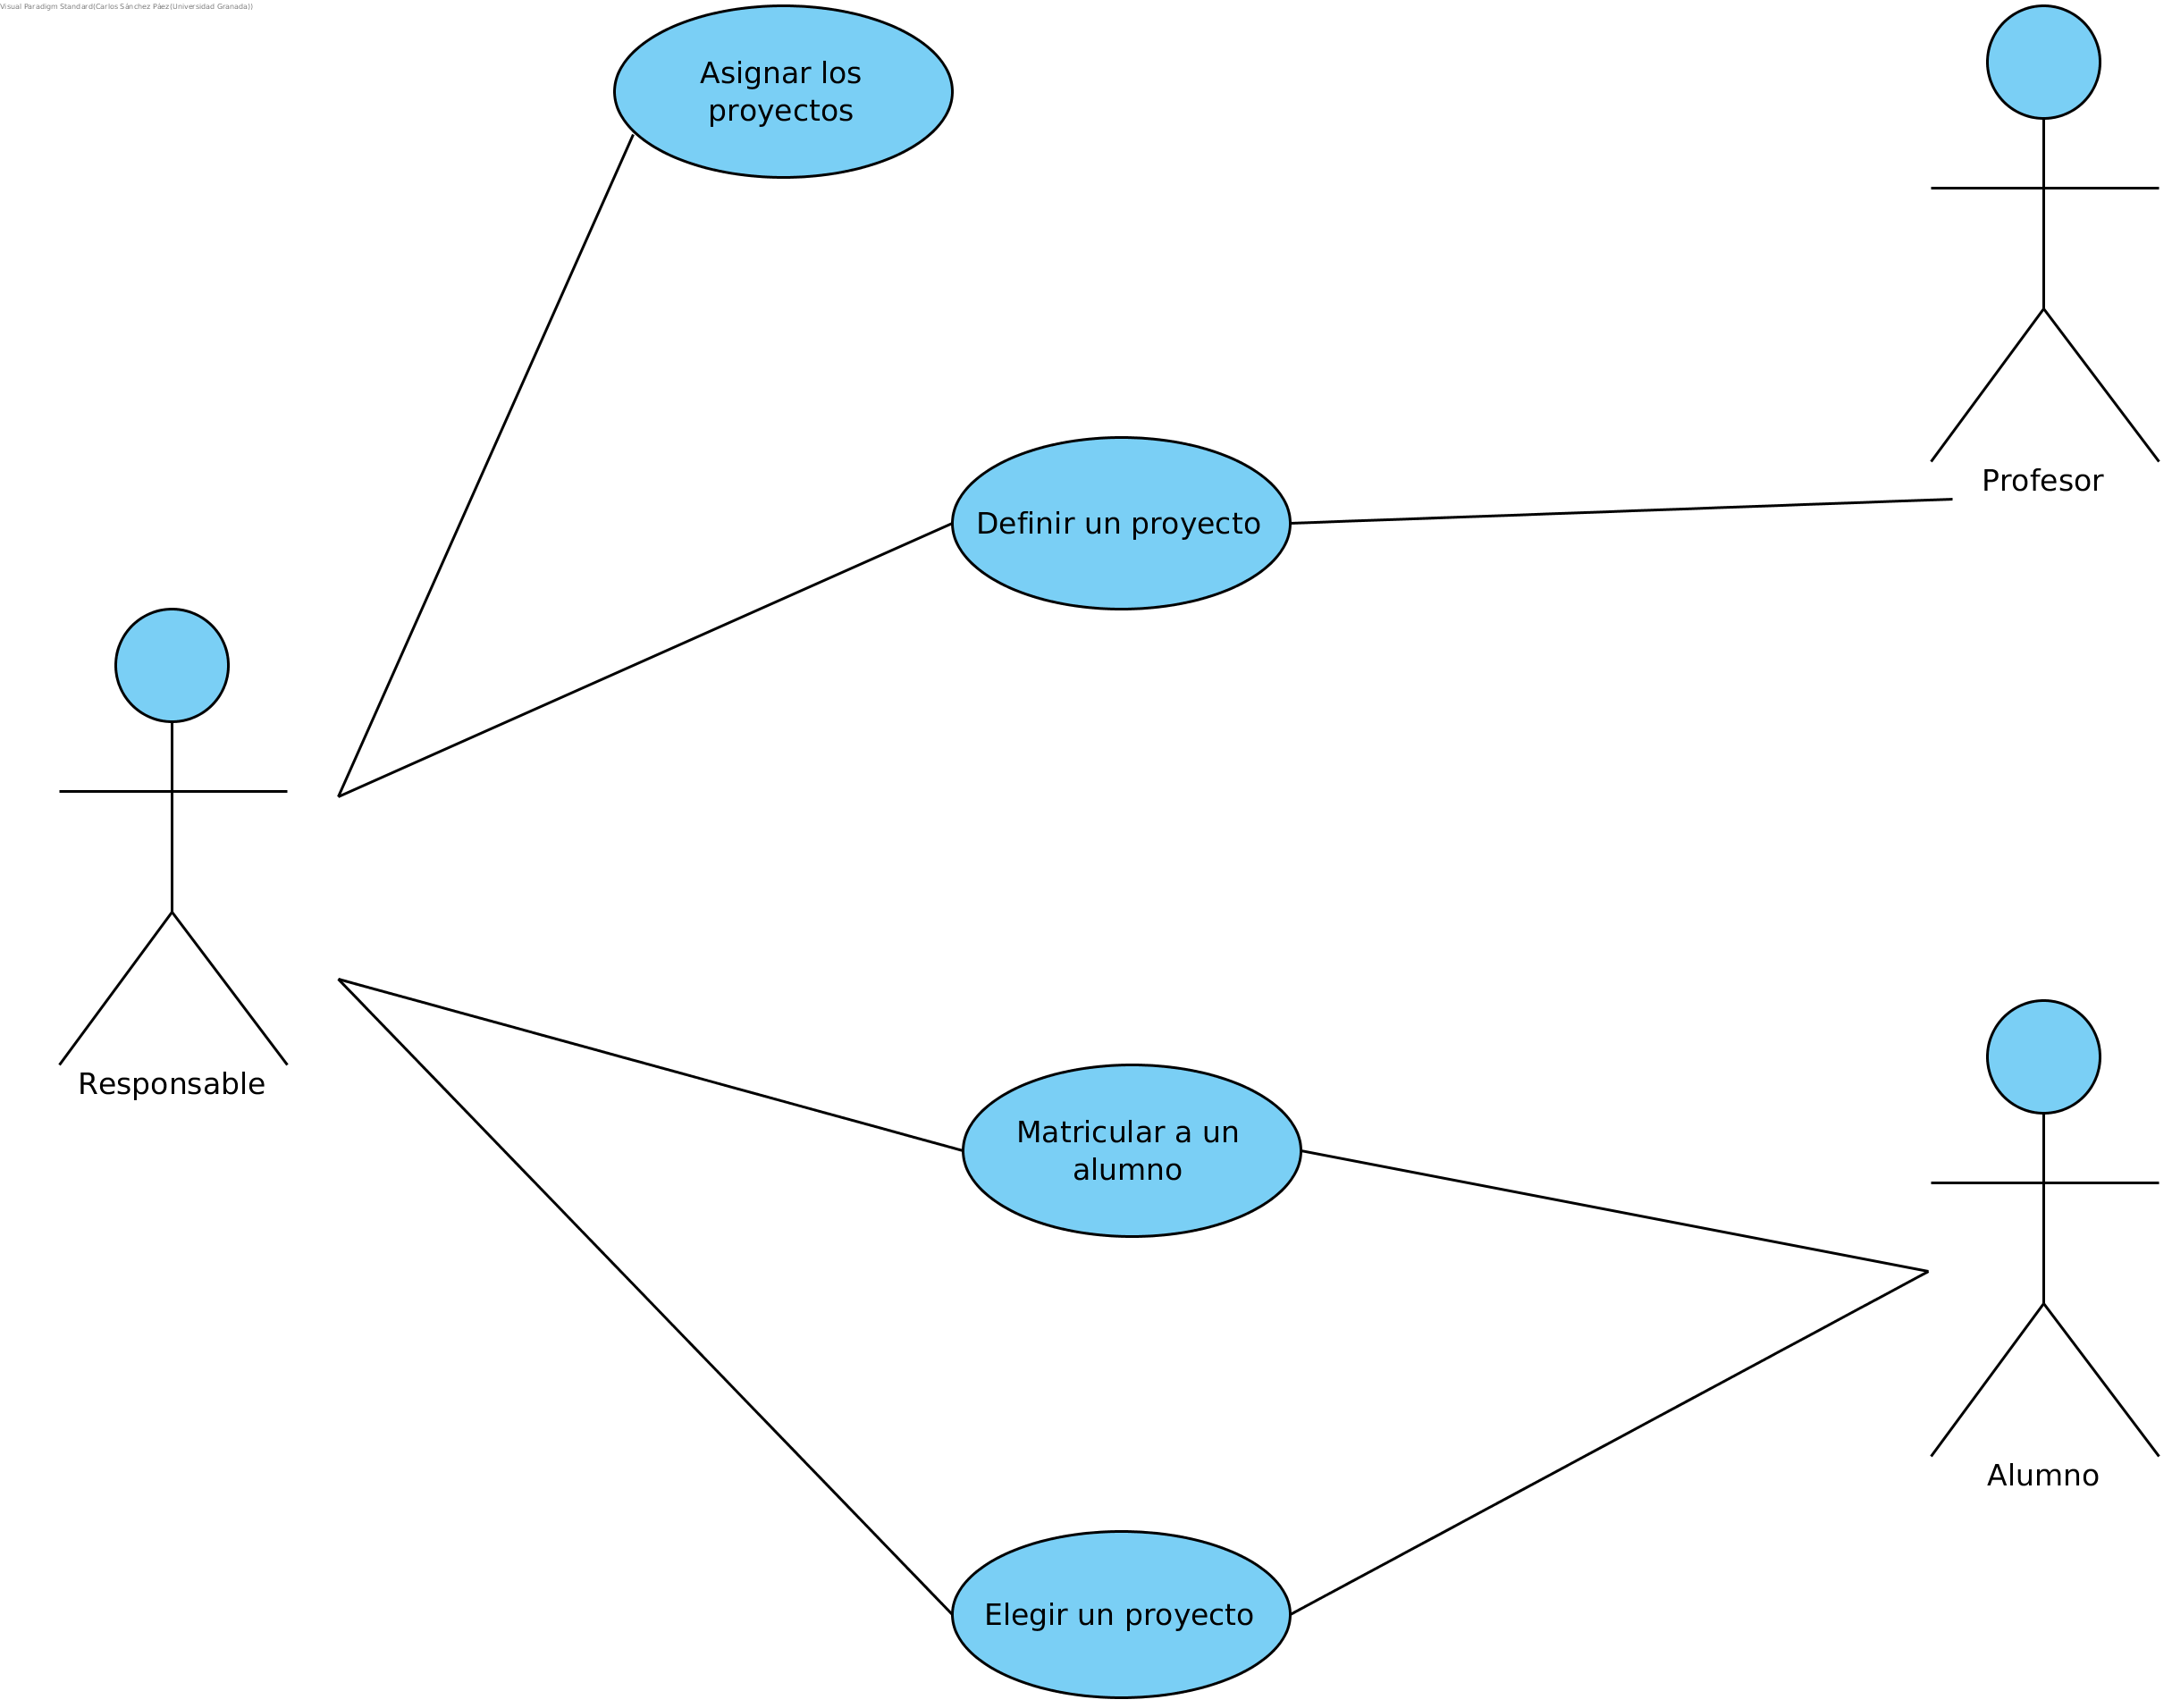
\includegraphics[scale=0.5]{cu_ej.png}
	\caption{Ejemplo de un caso de uso (gestión de proyectos).}
\end{figure}
\newpage
\subsubsection{Descripción del actor}

Para describir a un actor utilizaremos la siguiente plantilla: 
\begin{figure}[H]
\centering
\begin{tabular}{|m{3cm}|m{4cm}|m{2cm}|m{2cm}|m{2cm}|m{1cm}|}
\hline
\textbf{Actor} &  \multicolumn{4}{m{8cm}|}{\textit{Nombre el actor.}} &  \cellcolor{gray!40}\textit{ID} \\
\hline
\textbf{Descripción} & \multicolumn{5}{m{8cm}|}{\textit{Breve descripción del actor.}} \\
\hline
\textbf{Características} & \multicolumn{5}{m{8cm}|}{\textit{Características que describen al actor.}} \\
\hline
\textbf{Relaciones} &\multicolumn{5}{m{8cm}|}{\textit{Relaciones que posee el actor con otros actores del sistema.}} \\
\hline
\textbf{Referencias} & \multicolumn{5}{m{8cm}|}{\textit{Elementos del desarrollo en los que interviene el actor (casos de uso, diagramas, etc.)}} \\
\hline
\textbf{Autor} &  & \textbf{Fecha} &  & \textbf{Versión} &  \\
\hline
\end{tabular}

\vspace{0.5cm}

\begin{tabular}{|m{4cm}|m{7.3cm}|m{4cm}|}
\hline
\multicolumn{3}{|m{15.3cm}|}{\textbf{Atributos}} \\
\hline
\textbf{Nombre} & \textbf{Descripción} & \textbf{Tipo} \\
 \hline
... & ... & ... \\
\hline
\multicolumn{3}{|m{15.3cm}|}{\textit{Atributos principales del actor.}} \\
\hline
\end{tabular}

\vspace{0.5cm}

\begin{tabular}{|m{16.2cm}|}
\hline
\textbf{Comentarios} \\
\hline
\textit{Comentarios adicionales sobre el actor.} \\
\hline
\end{tabular}

\caption{Plantilla para la descripción de un actor}

\end{figure}

\begin{figure}[H]
\centering
\begin{tabular}{|m{3cm}|m{4cm}|m{2cm}|m{2cm}|m{2cm}|m{1cm}|}
\hline
\textbf{Actor} &  \multicolumn{4}{m{8cm}|}{Profesor} & \cellcolor{gray!40} \textit{ACT1} \\
\hline
\textbf{Descripción} & \multicolumn{5}{m{8cm}|}{Profesor que tutoriza algún proyecto de la asignatura TFG} \\
\hline
\textbf{Características} & \multicolumn{5}{m{8cm}|}{Puede ser cualquier profesor perteneciente a la ETSIIT.} \\
\hline
\textbf{Relaciones} &\multicolumn{5}{m{8cm}|}{\textit{-}} \\
\hline
\textbf{Referencias} & \multicolumn{5}{m{8cm}|}{CU1 (Definir proyecto)} \\
\hline
\textbf{Autor} & LSI & \textbf{Fecha} & - & \textbf{Versión} & - \\
\hline
\end{tabular}

\vspace{1cm}

\begin{tabular}{|m{4cm}|m{7.3cm}|m{4cm}|}
\hline
\multicolumn{3}{|m{15.3cm}|}{\textbf{Atributos}} \\
\hline
\textbf{Nombre} & \textbf{Descripción} & \textbf{Tipo} \\
\hline
Datos personales & Nombre, DNI, correo, etc. & Lista de cadenas de caracteres. \\
 \hline
Departamento & Nombre del departamento al que pertenece & Cadenas de caracteres. \\
\hline
Lista de proyectos & Trabajos que oferta para realizar. &  \\
\hline

\end{tabular}

\vspace{1cm}

\begin{tabular}{|m{16.2cm}|}
\hline
\textbf{Comentarios} \\
\hline
- \\
\hline
\end{tabular}

\caption{Ejemplo: descripción del actor profesor.}

\end{figure}

\subsubsection{Descripción del Caso de Uso}

\paragraph{Contenido}

La descripción de un caso de uso comprende:
\begin{itemize}
	\item \textbf{Inicio}. Cuándo y qué actor lo produce.
	\item \textbf{Fin}. Cuándo se produce y qué se obtiene.
	\item \textbf{Interacción}. Para qué se usa o qué intenta el caso de uso.
	\item \textbf{Cronología} y origen de las interacciones.
	\item \textbf{Repeticiones de comportamiento}. Qué acciones se repiten.
	\item \textbf{Situaciones opcionales o de error}. Qué situaciones alternativas se presentan en el caso de uso.
\end{itemize}

\paragraph{Tipos de casos de uso}

\begin{itemize}
	\item Dependiendo del \textbf{procesamiento}:
		\begin{itemize}
			\item \textbf{Básico}. Descripción general del procesamiento.
			\item \textbf{Extendido}. Descripción de la secuencia de acción completa entre actores y sistema.
		\end{itemize}	
	\begin{figure}[H]
		\centering
		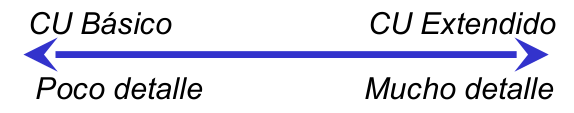
\includegraphics[scale=0.35]{cu_basico_extendido.png}
		\caption{Diferencia entre caso de uso básico y extendido.}
	\end{figure}
	\item Dependiendo de su \textbf{nivel de abstracción}:
		\begin{itemize}
			\item \textbf{Esencial}. Expresado de forma abstracta, contiene poca tecnología y pocos detalles de diseño.
			\item \textbf{Real}. Expresado en base al diseño actual. Aparecen relaciones con la \emph{interfaz de usuario}.
		\end{itemize}
	\begin{figure}[H]
		\centering
		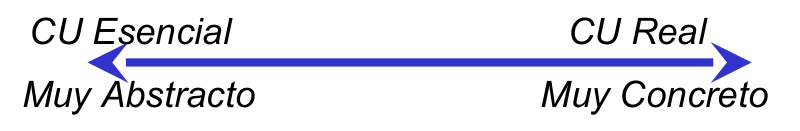
\includegraphics[scale=0.3]{cu_real_esencial.png}
		\caption{Diferencia entre caso de uso real y esencial.}
	\end{figure}
			
\end{itemize}

\paragraph{Plantilla básica}
La plantilla básica para casos de uso es la siguiente: 
\begin{figure}[H]
\centering
\begin{tabular}{|m{3cm}|m{2.65cm}|m{2cm}|m{2cm}|m{2cm}|m{1cm}|}
\hline
\textbf{Caso de uso} &  \multicolumn{4}{m{9.65cm}|}{\textit{Nombre del caso de uso}} &  \cellcolor{gray!40}ID \\
\hline
\textbf{Actores} & \multicolumn{5}{m{9.65cm}|}{\textit{Actores que participan en el caso de uso, indicando si son principales o secundarios.}} \\
\hline
\textbf{Tipo} & \multicolumn{5}{m{9.65cm}|}{\textit{Tipo de caso de uso.}} \\
\hline
\textbf{Referencias} &\multicolumn{3}{m{4.77cm}|}{\textit{Requisitos funcionales}} & \multicolumn{2}{m{4.77cm}|}{\textit{Casos de uso}} \\
\hline
\textbf{Precondición} & \multicolumn{5}{m{9.65cm}|}{\textit{Condiciones sobre el estado del sistema que deben cumplirse para que se pueda realizar el caso de uso.}} \\
\hline
\textbf{Postcondición} & \multicolumn{5}{m{9.65cm}|}{\textit{Efectos que tiene la realización del caso de uso sobre el sistema.}} \\
\hline
\textbf{Autor} & - & \textbf{Fecha} & - & \textbf{Versión} & - \\
\hline
\end{tabular}

\vspace{1cm}

\begin{tabular}{|m{16.2cm}|}
\hline
\textbf{Propósito} \\
\hline
\textit{Descripción del objetivo que cubre el caso de uso (una línea).} \\
\hline
\end{tabular}

\vspace{1cm}

\begin{tabular}{|m{16.2cm}|}
\hline
\textbf{Resumen} \\
\hline
\textit{Descripción a alto nivel de la secuencia de acciones realizadas en el caso de uso (un párrafo).} \\
\hline
\end{tabular}

\caption{Plantilla básica para casos de uso}

\end{figure}


\begin{figure}[H]
\centering
\begin{tabular}{|m{3cm}|m{2.65cm}|m{2cm}|m{2cm}|m{2cm}|m{1cm}|}
\hline
\textbf{Caso de uso} &  \multicolumn{4}{m{9.65cm}|}{Elegir proyecto} &  \cellcolor{gray!40}CU05 \\
\hline
\textbf{Actores} & \multicolumn{5}{m{9.65cm}|}{Alumno (principal) y responsable (secundario)} \\
\hline
\textbf{Tipo} & \multicolumn{5}{m{9.65cm}|}{Primario y esencial.} \\
\hline
\textbf{Referencias} &\multicolumn{3}{m{4.77cm}|}{RF27 y RF31} & \multicolumn{2}{m{4.77cm}|}{CU01} \\
\hline
\textbf{Precondición} & \multicolumn{5}{m{9.65cm}|}{El alumno debe estar matriculado en la asignatura \textit{Proyectos informáticos}.} \\
\hline
\textbf{Postcondición} & \multicolumn{5}{m{9.65cm}|}{El alumno tendrá un proyecto más en su lista de proyectos elegidos.} \\
\hline
\textbf{Autor} & LSI & \textbf{Fecha} & -  & \textbf{Versión} & - \\
\hline
\end{tabular}

\vspace{1cm}

\begin{tabular}{|m{16.2cm}|}
\hline
\textbf{Propósito} \\
\hline
Permitir que el alumno pueda elegir un posible proyecto a realizar de entre los ofertados por los profesores. \\
\hline
\end{tabular}

\vspace{1cm}

\begin{tabular}{|m{16.2cm}|}
\hline
\textbf{Resumen} \\
\hline
El alumno informa que quiere seleccionar un proyecto, indica la prioridad con la que realiza la selección y se almacena su interés por el proyecto. \\
\hline
\end{tabular}

\caption{Ejemplo: plantilla básica del caso de uso elegir proyecto}

\end{figure}


\paragraph{Plantilla extendida}
Para la descripción extendida recurrimos a \emph{escenarios}.\\

Un \textbf{escenario} es una secuencia específica y concreta de acciones e interacciones entre los actores y el sistema objeto de estudio. \\

Los sistemas pueden ser:
\begin{itemize}
	\item \textbf{Básicos}. Situaciones normales y comunes de actuación.
	\item \textbf{Secundarios}. Se corresponden con situaciones alternativas y de error.
\end{itemize}

Consiste en añadir lo siguiente a la plantilla básica: 

\begin{figure}[H]
\centering
\begin{tabular}{|m{5pt}|m{7.33cm}|m{5pt}|m{7.33cm}|}
\hline
\multicolumn{4}{|c|}{\textbf{Curso normal}} \\
\hline
\multicolumn{2}{|c}{\textbf{Actor}} & \multicolumn{2}{|c|}{\textbf{Sistema}} \\
\hline
\textbf{1} & \textit{Acción realizada por un actor} & \textbf{2} & \textit{Acción realizada por el sistema.} \\
\hline
\textbf{..} & ... & \textbf{..} & ... \\
\hline
\textbf{\footnotesize{m}} & \textit{Acción realizada por un actor} & \textbf{..} & ... \\
\hline
\textbf{-} & ... & \textbf{n} & \textit{Acción realizada por el sistema.} \\
\hline

\end{tabular}

\vspace{0.5cm}

\begin{tabular}{|m{15pt}|m{7.15cm}|m{6pt}|m{7.15cm}|}
\hline
\multicolumn{4}{|m{16.2cm}|}{\textbf{Cursos alternos}} \\
\hline
\textbf{n.a} & \multicolumn{3}{l|}{\textit{Alternativa \emph{a} a la acción n del curso normal.}}  \\
\hline
\multicolumn{2}{|m{7.2cm}}{\textbf{Actor}} & \multicolumn{2}{|m{7.2cm}|}{\textbf{Sistema}} \\
\hline
1 & \textit{Acción del actor} & .. & ... \\
\hline
.. & ... & 2 & \textit{Acción del sistema} \\
\hline
.. & ... & .. & ... \\
\hline
\textbf{n.b} & \multicolumn{3}{l|}{\textit{Alternativa \emph{b} a la acción n del curso normal.}}  \\
\hline
.. & ... & .. & ... \\
\hline
\end{tabular}

\vspace{0.5cm}

\begin{tabular}{|m{3.75cm}|m{3.75cm}|m{3.75cm}|m{3.8cm}|}
\hline
\multicolumn{4}{|c|}{\textbf{Otros datos}} \\
\hline
\textbf{Frecuencia esperada} & \textit{Número de veces que se realiza el caso de uso por unidad de tiempo.} & \textbf{Rendimiento} & \textit{Rendimiento esperado.} \\
\hline
\textbf{Importancia} & \textit{Vital, alta, moderada o baja.} & \textbf{Urgencia} & \textit{Urgencia en su desarrollo.} \\
\hline
\textbf{Estado} & \textit{Estado de desarrollo actual.} & \textbf{Estabilidad} & \textit{Estabilidad de los requisitos asociados} \\
\hline
\end{tabular}

\vspace{1cm}

\begin{tabular}{|m{16.2cm}|}
\hline
\textbf{Comentarios} \\
\hline
\textit{Otros aspectos a aclarar.} \\
\hline
\end{tabular}

\caption{Plantilla extendida para casos de uso.}

\end{figure}

\begin{figure}[H]
\centering
\begin{tabular}{|m{5pt}|m{7.33cm}|m{5pt}|m{7.33cm}|}
\hline
\multicolumn{4}{|c|}{\textbf{Curso normal}} \\
\hline
\multicolumn{2}{|c}{\textbf{Actor}} & \multicolumn{2}{|c|}{\textbf{Sistema}} \\
\hline
\textbf{1} & El alumno solicita la lista de proyectos ofertados. & \textbf{2} & Proporciona la lista. \\
\hline
\textbf{3} & El alumno elige un proyecto determinado. & \textbf{4} & Solicita la prioridad con la que el alumno realiza la petición. \\
\hline
\textbf{4} & El alumno proporciona la prioridad deseada. & \textbf{6} & Almacena la elección realizada por el alumno e informa de que la operación ha sido realizada con éxito. \\
\hline
\end{tabular}

\vspace{0.5cm}

\begin{tabular}{|m{15pt}|m{7.15cm}|m{6pt}|m{7.15cm}|}
\hline
\multicolumn{4}{|m{16.2cm}|}{\textbf{Cursos alternos}} \\
\hline
\textbf{6.a} & \multicolumn{3}{l|}{El alumno proporciona una prioridad ya usada para otro proyecto.}  \\
\hline
\multicolumn{2}{|m{7.2cm}}{\textbf{Actor}} & \multicolumn{2}{|m{7.2cm}|}{\textbf{Sistema}} \\
\hline
.. & ... & 1 & El sistema informa de la situación y finaliza el caso de uso. \\
\hline
\textbf{6.b} & \multicolumn{3}{l|}{El alumno ha elegido más de 10 proyectos.}  \\
\hline
.. & ... & 1 & El sistema informa de la situación y finaliza el caso de uso. \\
\hline
\end{tabular}

\vspace{0.5cm}

\begin{tabular}{|m{3.75cm}|m{3.75cm}|m{3.75cm}|m{3.8cm}|}
\hline
\multicolumn{4}{|c|}{\textbf{Otros datos}} \\
\hline
\textbf{Frecuencia esperada} & 40 veces al año. & \textbf{Rendimiento} & No más de 5 minutos. \\
\hline
\textbf{Importancia} & Alta. & \textbf{Urgencia} & Alta. \\
\hline
\textbf{Estado} & Iniciando su desarrollo. & \textbf{Estabilidad} & Alta. \\
\hline
\end{tabular}

\vspace{1cm}

\begin{tabular}{|m{16.2cm}|}
\hline
\textbf{Comentarios} \\
\hline
El caso de uso se realizará por al menos 40 alumnos. \\
\hline
\end{tabular}

\caption{Ejemplo: plantilla extendida del caso de uso elegir proyecto.}

\end{figure}

\subsubsection{Relaciones de los Casos de Uso}

Las \emph{finalidades} de las relaciones son:
\begin{itemize}
	\item \textbf{Organizar} los casos de uso.
	\item Mejorar la \textbf{comprensión}.
	\item \textbf{Reducir la redundancia} del texto.
	\item \textbf{Mejorar la gestión} de los documentos generados.
\end{itemize}

\begin{figure}[H]
\centering
\begin{tabular}{|m{3cm}|m{6.5cm}|m{6cm}|}
\hline
\cellcolor{blue!30}Tipo de Relación & \cellcolor{blue!30}Definición & \cellcolor{blue!30}Notación \\
\hline
\textbf{Asociación} & Relación entre un actor y el caso de uso en el que participa. &
\begin{center}
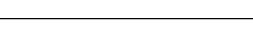
\includegraphics[scale=0.5]{asociacion_uml.png}
\end{center} \\
\hline
\textbf{Extensión} & Relación entre casos de uso. Representa la inserción de fragmentos de comportamiento adicional sin que el caso de uso base conozca los casos de uso de extensión &
\begin{center}
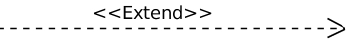
\includegraphics[scale=0.4]{extension_uml.png}
\end{center} \\
\hline
\textbf{Generalización} & Relación entre un caso de uso general y otro específico, que hereday añade características al caso de uso general. &
\begin{center}
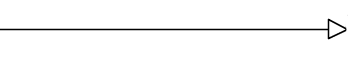
\includegraphics[scale=0.4]{generalizacion_uml.png}
\end{center} \\
\hline
\textbf{Inclusión} & Relación entre casos de uso. Representa la inserción de comportamiento adicional dentro del caso de uso base. Hace referencia explícita al caso de uso de inclusión. & 
\begin{center}
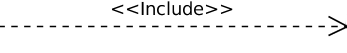
\includegraphics[scale=0.4]{inclusion_uml.png}
\end{center}\\
\hline
\end{tabular}
\caption{Tipos de relaciones entre casos de uso}
\end{figure}

\paragraph{Relación de inclusión}

Sus características son las siguientes:
\begin{itemize}
	\item Es una \textbf{relación de dependencia} entre dos casos de uso que permite \emph{incluir el comportamiento} de un caso de uso en el flujo de otro.
	\item El caso de uso que incluye se denomina \emph{caso de uso base} y el incluido \emph{caso de uso de inclusión}.
	\item El caso de uso base se realiza hasta que se alcanza el punto donde se encuentra la referencia al caso de uso de inclusión, donde la ejecución pasa al caso de uso de inclusión. Cuando éste termina, el control regresa al caso de uso base.
	\item El caso de uso de inclusión se utiliza \emph{completamente} por el caso de uso base.
	\item El caso de uso base \emph{no está completo} sin todos sus casos de uso de inclusión.
	\item El caso de uso de inclusión puede ser \emph{compartido} por varios casos de uso base.
	\item El caso de uso de inclusión \emph{no es opcional} y es necesario para que tenga sentido el caso de uso base.
\end{itemize}

\begin{figure}[H]
\centering
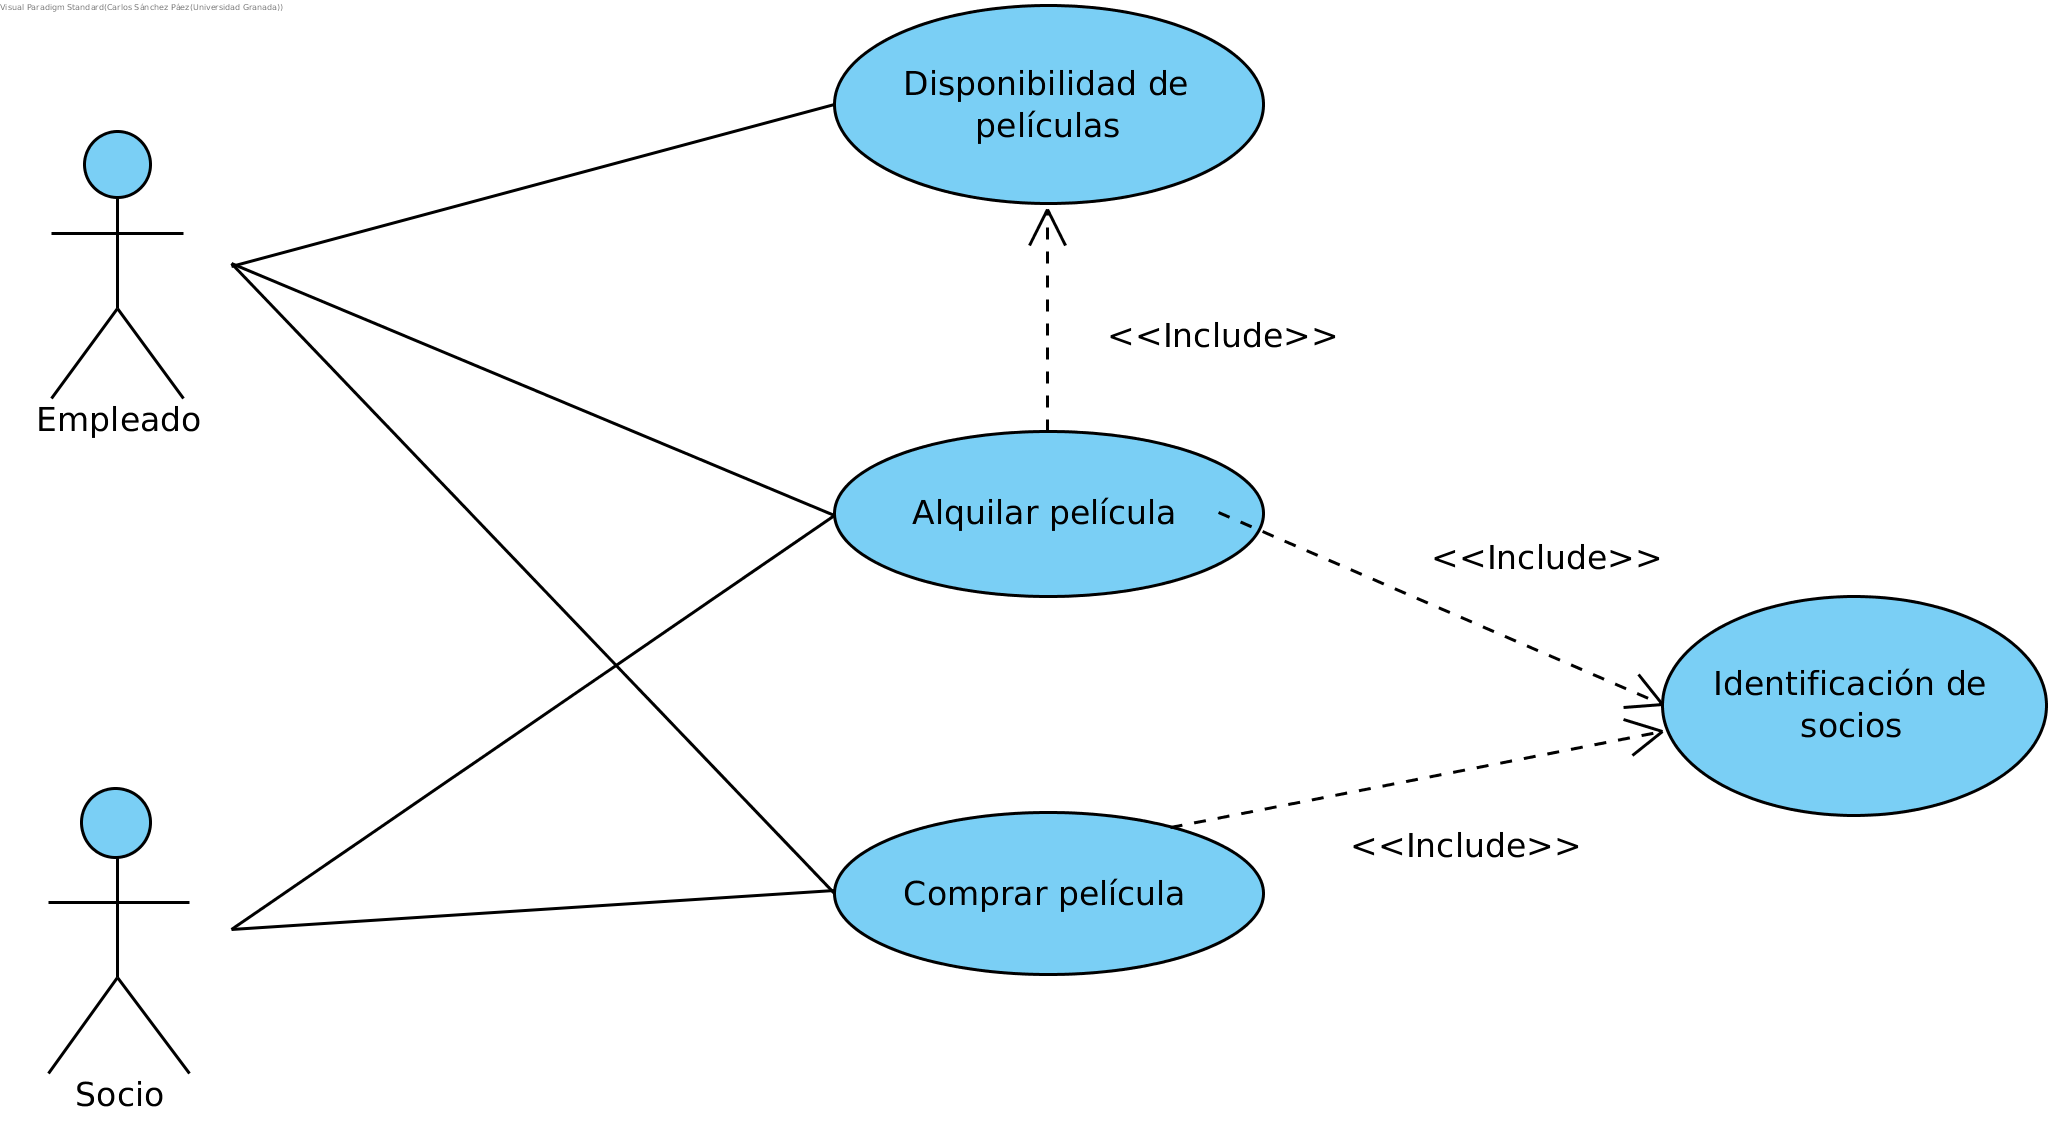
\includegraphics[scale=0.75]{ej_inclusion.png}
\caption{Ejemplo de inclusión en un diagrama.}
\end{figure}


\begin{figure}[H]
\centering
\begin{tabular}{|m{10pt}|m{7cm}|m{10pt}|m{7cm}|}
\hline
\multicolumn{4}{|c|}{\textbf{Curso normal}} \\
\hline
\multicolumn{2}{|c}{\textbf{Actor}} & \multicolumn{2}{|c|}{\textbf{Sistema}} \\
\hline
\textbf{1} & El socio solicita el alquiler de una película. &  & \\
\hline
\textbf{2} & El socio proporciona sus datos de socio. &  &  \\
\hline
\textbf{3} & El empleado identifica al socio. & \textbf{4} & \textbf{incluir(CU12. Identificación de socio)} \\
\hline
\textbf{5} & El socio proporciona el título de la película a alquilar. &  &  \\
\hline
\textbf{5} & El empleado identifica la película y pide registro del alquiler. & \textbf{7} & \textbf{incluir(CU17. Disponibilidad de películas)}. \\
\hline
 & & \textbf{8} & Guarda los datos del alquiler.  \\
\hline
 & & \textbf{8} & Informa de la cantidad a pagar.  \\
\hline
\textbf{10} & El empleado informa al socio de la cantidad a pagar. &  &  \\
\hline
\textbf{11} & Realiza el pago del alquiler. & \textbf{12} & Genera el resguardo de alquiler. \\
\hline
\textbf{10} & El empleado entrega el resguardo al socio. &  &  \\
\hline
\end{tabular}
\caption{Ejemplo de inclusión en la descripción de un caso de uso (alquilar película)}
\end{figure}

\paragraph{Relación de extensión}

Sus características son:

\begin{itemize}
	\item Es una \emph{relación de dependencia} que especifica que el comportamiento del caso de uso base puede ser extendido por otro caso de uso (caso de uso de extensión) bajo determinadas condiciones.
	\item El caso de uso base declara uno o más \emph{puntos de extensión} que son "anclajes" en los que se pueden añadir nuevos comportamientos.
	\item El caso de uso de extensión define \emph{segmentos de inserción}, que pueden ser insertados en los puntos de enganche cuando se cumpla una determinada condición.
	\item El \emph{caso de uso base} no sabe nada de los casos de uso de extensión y \emph{está completo sin ellos}. De hecho, los puntos de extensión no están numerados en el flujo de eventos del caso de uso base.
	\item El caso de uso de extensión no tiene sentido sin el caso de uso base.
\end{itemize}

\begin{figure}[H]
	\centering
	\begin{subfigure}[b]{0.25\textwidth}
		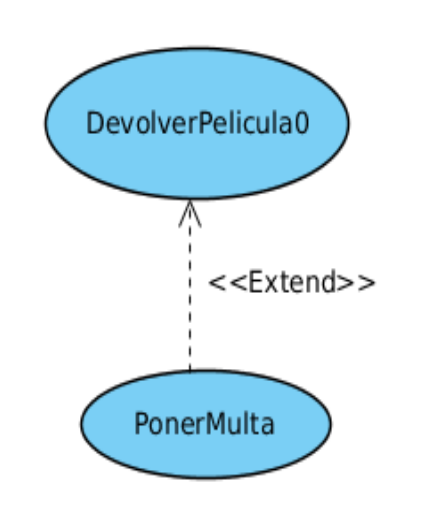
\includegraphics[width=\textwidth]{extension_basica.png}
		\caption{Notación básica}
	\end{subfigure}
	\quad
	\begin{subfigure}[b]{0.3\textwidth}
		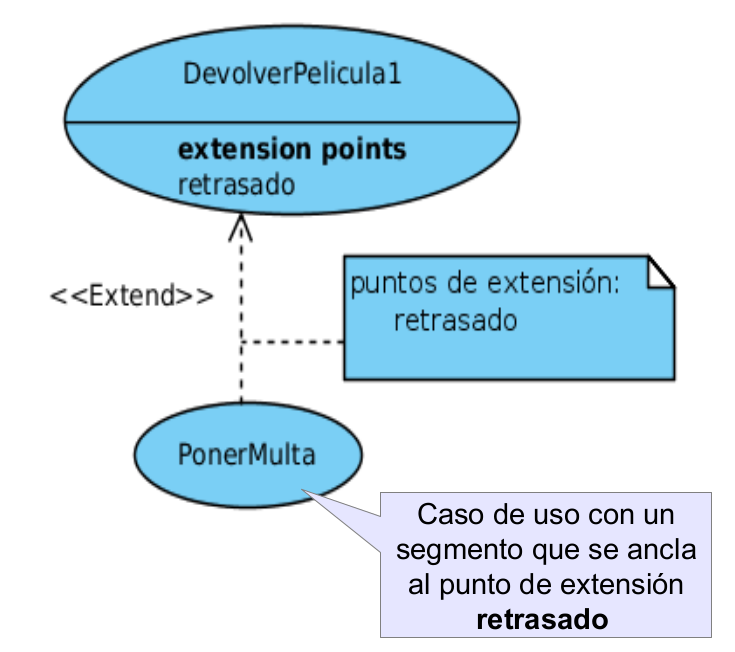
\includegraphics[width=\textwidth]{extension_extendida.png}
		\caption{Notación extendida}
	\end{subfigure}
	\vskip 0.5cm
	\begin{subfigure}[b]{0.5\textwidth}
		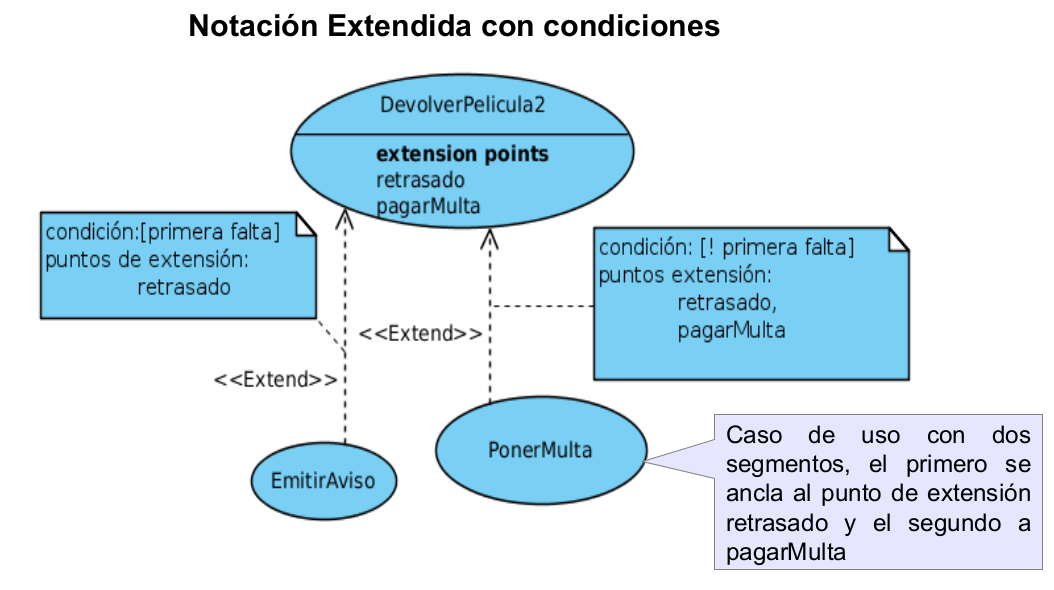
\includegraphics[width=\textwidth]{extension_condiciones.png}
		\caption{Notación extendida con condiciones}
	\end{subfigure}
	\caption{Distintas notaciones de la relación de extensión.}
\end{figure}

\begin{figure}[H]
\centering
\begin{tabular}{|m{10pt}|m{7cm}|m{10pt}|m{7cm}|}
\hline
\multicolumn{4}{|c|}{\textbf{Curso normal}} \\
\hline
\multicolumn{2}{|c}{\textbf{Actor}} & \multicolumn{2}{|c|}{\textbf{Sistema}} \\
\hline
\textbf{1} & El socio solicita devolver de una película. &  & \\
\hline
\textbf{2} & El socio proporciona sus datos de socio. &  &  \\
\hline
\textbf{3} & El empleado identifica al socio. & \textbf{4} & incluir(CU12. Identificación de socio) \\
\hline
\textbf{5} & El socio proporciona el título de la película a devolver. &  &  \\
\hline
 & \textbf{Punto de extensión: retrasado} & & \\
 \hline
\textbf{6} & El empleado incluye la película devuelta. & \textbf{7} & Almacena la devolución. \\
\hline
  & \textbf{Punto de extensión: pagarMulta}. & &   \\
\hline
 & & \textbf{8} & El empleado proporciona justificante de devolución.  \\
\hline
\end{tabular}
\caption{Ejemplo de extensión en la descripción de un caso de uso (devolver película)}
\end{figure}

\begin{figure}[H]
\centering
\begin{tabular}{|c|c|c|c|}
\hline
\multicolumn{2}{|c|}{\textbf{Caso de uso de extensión}} & \multicolumn{2}{c|}{Emitir aviso} \\
\hline
\multicolumn{2}{|c|}{\textbf{Segmento}} & \multicolumn{2}{c|}{1}\\
\hline
\multicolumn{2}{|c|}{\textbf{Precondición}} & \multicolumn{2}{c|}{Devolución fuera de plazo.}\\
\hline
\end{tabular}
\vskip 0.5 cm
\begin{tabular}{|c|c|c|c|}
\hline
\multicolumn{4}{|c|}{\textbf{Curso normal de eventos}} \\
\hline
\multicolumn{2}{|c|}{\textbf{Actor}} & \multicolumn{2}{c|}{\textbf{Sistema}}\\
\hline
1 & El empleado incorpora los detalles del aviso. & 2 & Almacena el aviso.\\
\hline
3 & El empleado le indica al socio que tiene un aviso por retraso. & & \\
\hline
\end{tabular}
\caption{Ejemplo de descripción de un caso de uso de extensión (emitir aviso)}
\end{figure}


Para usar correctamente estas relaciones debemos:
\begin{itemize}
	\item Usar relaciones de \emph{extensión} para comportamientos excepcionales, opcionales o que rara vez suceden.
	\item Usar relaciones de \emph{inclusión} para comportamientos que se comparten entre dos o más casos de uso, o bien para separar un caso de uso en subunidades.
\end{itemize}

\paragraph{Relación de generalización}

\begin{itemize}
	\item Es una relación entre un caso de uso general (\emph{padre}) y otros más especializados (\emph{hijos}).
	\item Los casos de uso hijos:
		\begin{itemize}
			\item Heredan todas las características del caso de uso general.
			\item Pueden añadir nuevas características.
			\item Pueden anular o reescribir características del caso de uso general, salvo relaciones, puntos de extensión y precondiciones.
		\end{itemize}
\end{itemize}

\begin{figure}[H]
\centering
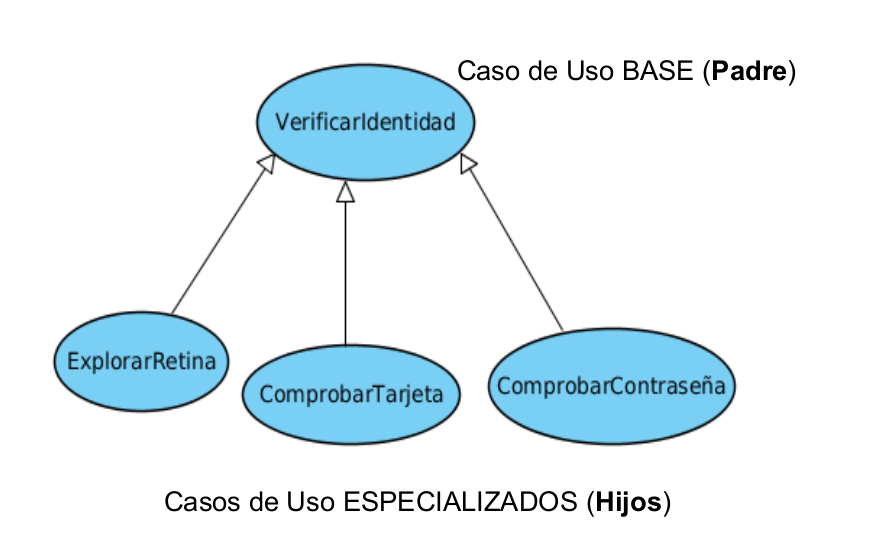
\includegraphics[scale=0.35]{notacion_generalizacion.png}
\caption{Notación UML de la relación de generalización.}
\end{figure}

En cuanto a la descripción de los casos de uso hijos no hay diferencia con respecta a cualquier otro caso de uso.

\begin{figure}[H]
\centering
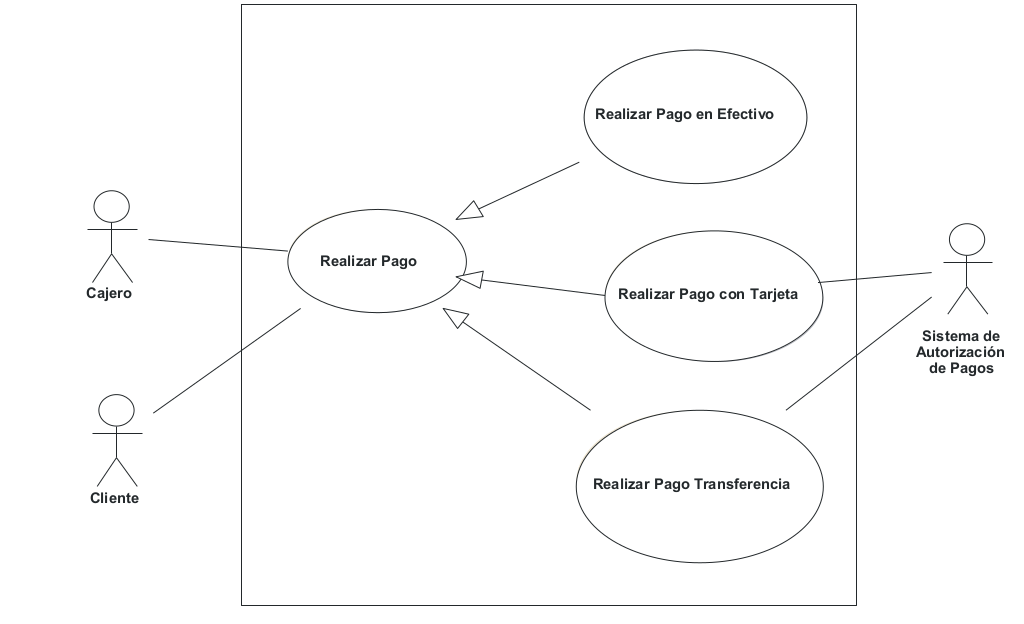
\includegraphics[scale=0.4]{generalizacion_ej.png}
\caption{Ejemplo de generalización.}
\end{figure}

\paragraph{Recomendaciones de uso de las relaciones entre casos de uso}

\begin{itemize}
	\item Usar las relaciones entre casos de uso cuando \emph{simplifiquen el modelo}.
	\item Un sencillo modelo de casos de uso es preferible a uno con demasiadas relaciones, ya que son más fáciles de entender.
	\item El uso de muchas relaciones de inclusión hace que tengamos que ver más de un caso de uso para tener una idea completa.
	\item Las relaciones de extensión son complejas y difícules de entender por la comunidad de usuarios y clientes.
	\item La \emph{generalización} de casos de uso debería evitarse.
\end{itemize}
\subsubsection{Proceso de construcción del modelo de Casos de Uso}

Los pasos a seguir son los siguientes:
\begin{enumerate}
	\item Identificar actores (\emph{principales} y secundarios).
	\item Identificar los principales casos de uso de cada actor, identificando sus objetivos y necesidades, para lo que nos preguntamos:
		\begin{enumerate}
			\item ¿Cuáles son las \emph{tareas principales} que realiza cada actor?
			\item ¿Qué \emph{información del sistema} debe adquirir, producir o cambiar?
			\item ¿El actor tiene que informar sobre cambios producidos en el \emph{exterior del sistema}?
			\item ¿Qué información desea \emph{adquirir} el actor del sistema?
			\item ¿Desea el actor ser informado de \emph{cambios producidos} en el sistema?
		\end{enumerate}
	\item Identificar nuevos casos de uso a partir de los existentes, para lo que se deben analizar las siguientes situaciones:
		\begin{enumerate}
			\item Variaciones significativas de los casos de uso existentes.
			\item Acciones opuestas $\rightarrow$ casos de uso opuestos a los existentes.
			\item Acciones que deben realizarse antes o después de un caso de uso existente.
		\end{enumerate}
		\item Elaborar los diagramas de casos de uso y de paquetes en los que se muestren las relaciones lógicas entre diagramas de casos de uso.
		\item Confeccionar la descripción básica de cada caso de uso.
		\item Definir prioridades y seleccionar casos de uso primarios, teniendo en cuenta:
			\begin{itemize}
				\item Requisitos imprescindibles.
				\item Requisitos importantes.
				\item Requisitos deseables.
			\end{itemize}
		\item Realizar la descripción extendida de cada caso de uso.
		\item Elaborar los diagramas de actividad.
		\item Desarrollar prototipos de la interfaz de usuario.
\end{enumerate}
\subsubsection{Otros aspectos del modelo de Casos de Uso}

\paragraph{Diagrama de paquetes}
Es un diagrama UML usado para describir la estructura de un sistema mediante agrupaciones lógicas. También muestra las dependencias entre estas agrupaciones.\\
El diagrama de paquetes se utiliza en el modelado de casos de uso para agrupar de forma lógica los distintos diagramas de casos de uso.

\begin{figure}[H]
\centering
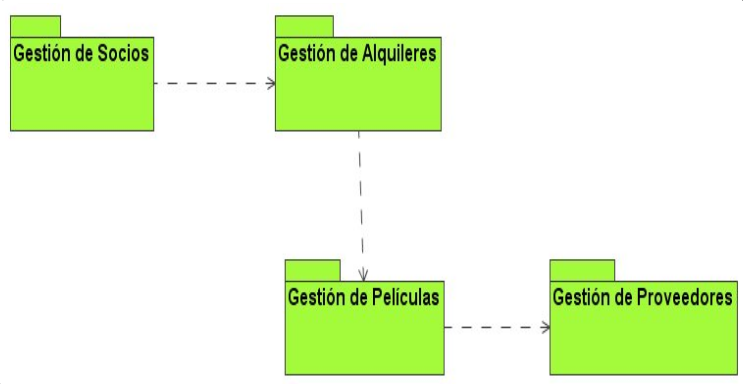
\includegraphics[scale=0.4]{diagrama_paquetes.png}
\caption{Diagrama de paquetes.}
\end{figure}

\paragraph{Diagrama de actividad}

Es un diagrama UML que describe el comportamiento que tienen una serie de tareas o procesos. Representan:
\begin{itemize}
	\item Los flujos de actividades de los procesos de negocio de una empresa.
	\item Los flujos de acciones de uno o varios casos de uso de forma gráfica.
\end{itemize}

\begin{figure}[H]
\centering
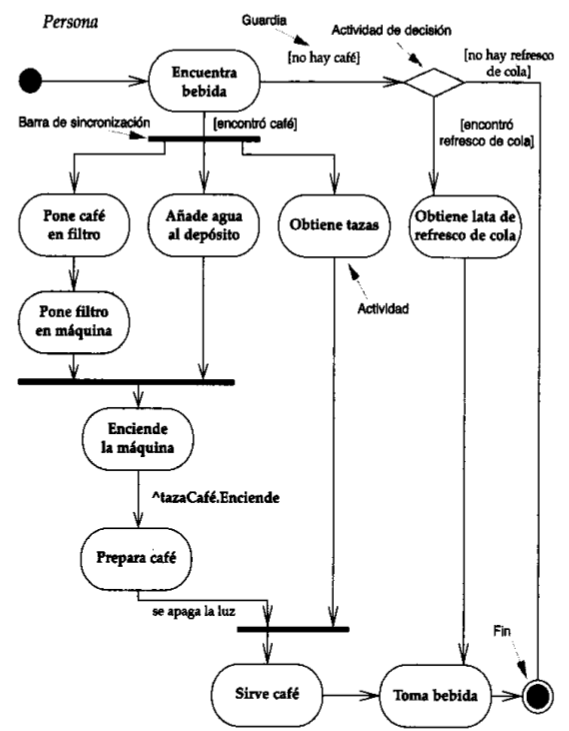
\includegraphics[scale=0.4]{diagrama_actividad.png}
\caption{Diagrama de actividad.}
\end{figure}

\newpage

\subsection{Análisis y especificación de requisitos}

\subsubsection{Introducción}

El proceso de análisis se ha usado tradicionalmente como un sinónimo de \emph{Ingeniería de Requisitos}. Sin embargo, en realidad se trata de una de sus fases, en la que hay que:

\begin{itemize}
	\item Descubrir los conflictos existentes entre los requisitos.
	\item Profundizar en el conocimiento del sistema (realizando modelos que sirvan de base para el diseño e implementación y sean más fáciles de entender por desarrolladores).
	\item Aumentar la formalización del conocimiento existente sobre el sistema para facilitar el mantenimiento.
\end{itemize}

El objetivo principal del análisis es refinar, estructurar y describir los requisitos para conseguir una comprensión más precisa y fácil de mantener que nos ayude a estructurar el sistema completo mediante modelos de análisis. Es importante rastrear los requisitos de usuario a través de los requisitos del software.

\paragraph{Ejemplo de estudio de soluciones.\\}

\textbf{Problema}. Llevar un control de los productos que se tienen en un almacén y realizar pedidos cuando sea necesario.\\

Posibles soluciones:

\begin{enumerate}
	\item Incluir una función en el sistema para obtener un listado de las existencias del almacén de cada producto. El almacenista pedirá los productos de los que haya pocas existencias.
	\item Incluir información sobre los mínimos necesarios para cada producto y una función para obtener un listado de los productos bajo mínimo.
	\item Incluir información sobre los proveedores de los productos y permitir que el sistema evalue los mínimos cada cierto tiempo, generando listados con los pedidos.
	\item Generar los pedidos por FAX de forma automática en base a la información de los proveedores y a los mínimos del almacén.
\end{enumerate}

\begin{figure}[H]
\centering
\begin{tabular}{|m{7.5cm}|m{7.5cm}|}
\hline
\textbf{Modelo CU}. & \textbf{Modelo de análisis}. \\
\hline
Lenguaje del cliente. & Lenguaje del desarrollador.\\
\hline
Vista externa del sistema estructurado en CU. & Vista interna del sistema estructurado en clases y subsistemas.\\
\hline
Contrato cliente/desarrolladores. & Con vistas a la solución.\\
\hline
Puede contener redundancias e inconsistencias entre requisitos. & No debe contenerlas.\\
\hline
Captura la funcionalidad del sistema & Esboza cómo llevar a cabo la funcionalidad (primera aproximación a la arquitectura).
\\
\hline
Se definen CU que serán analizados en mayor profundidad & Define realaciones entre casos de uso.\\
\hline
\end{tabular}
\caption{Diferencias entre modelos.}
\end{figure}

\subsubsection{Análisis orientado a objetos (AOO)}

El análisis orientado a objetos examina y representa los requisitos desde la perspectiva de los objetos que nos encontramos en el dominio del problema.\\

Hay una gran variedad de métodos AOO, aunque todos se centran en la obtención de modelos estáticos (de estructura) y dinámicos (de comportamiento).\\

El lenguaje más utilizado para representar estos modelos es UML.\\

El análisis orientado a objetos se usa por los siguientes motivos:
 
\begin{itemize}
	\item Los términos usados en los modelos están cercanos a los del mundo real, por lo que facilita y mejora la obtención de requisitos y acerca el espacio del problema al de la solución.
	\item Se modelan tanto elementos y propiedades estáticas como dinámicas.
	\item Manejamos conceptos comunes durante el análisis, diseño e implementación del software.
\end{itemize}

\subsubsection{Modelos del AOO}

\subsubsection{Modelo estático. Diagrama conceptual}

\begin{itemize}
	\item También se le conoce como diagrama de conceptos, diagrama de análisis, diagrama conceptual, modelo conceptual, modelo del dominio, etc.
	\item En él se representan los principales conceptos del dominio del problema, sus propiedades y las relaciones entre ellos. 
	\item El modelo de casos de uso es la base para obtener la información necesaria para el modelo estático.
	\item Se representa mediante diagramas de UML.
		\begin{itemize}
			\item Clases = conceptos del dominio del problema.
			\item Asociaciones entre conceptos.
			\item Generalizaciones de conceptos.
			\item Atributos de los conceptos.
		\end{itemize}
\end{itemize}

Los pasos que hay que seguir para su obtención son los siguientes:

\begin{enumerate}
	\item Identificar e incorporar \textbf{conceptos}.
	\item Identificar e incorporar \textbf{asociaciones} entre conceptos.
	\item Identificar e incorporar \textbf{generalizaciones} de conceptos.
	\item Identificar e incorporar \textbf{atributos} de conceptos.
	\item Estructurar y empaquetar el modelo.
	\end{enumerate}
	
\begin{figure}[H]
\centering
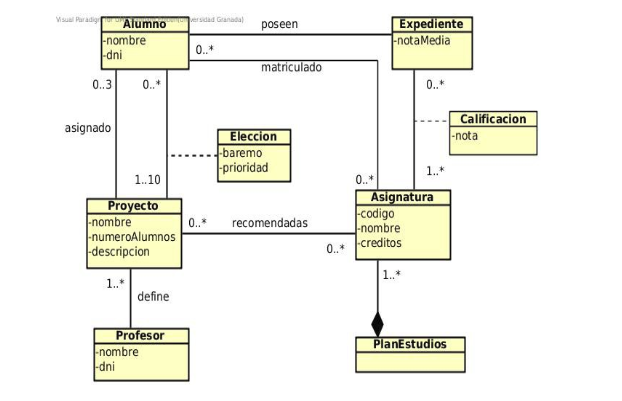
\includegraphics[scale=0.75]{ejemplo_estatico.png}
\caption{Ejemplo de modelo estático.}
\end{figure}

\subsubsection{Modelo de comportamiento}

Es un estudio adicional del dominio del problema en el que añadimos los requisitos funcionales al modelo del análisis.
\paragraph{Diagramas de secuencia del sistema (DSS).\\}

Es un diagrama de secuencia UML en el que sde muestran como los eventos generados por los actores van a provocar la ejecución de una operación por el Sistema, siendo visto como una caja negra.

Para elaborarlos debemos seguir los siguientes pasos:

\begin{enumerate}
	\item Identificar los \textbf{actores} que inician dichas operaciones.
	\item Asignar un nombre a todo el sistema.
	\item Identificar y nombrar las operaciones principales del sistema de las descripciones de los casos de uso.
	\item Ver cuales serían los parámetros de las operaciones.
	\item Representarlas en el diagrama de secuencia del sistema (DSS).
	\item Incluir las operaciones en la clase que identifica a todo el sistema del diagrama conceptual.
\end{enumerate}

Podemos tener un DSS para cada CU, un solo DSS con todas las operaciones del sistema o bien un DSS por cada diagrama de CU.

\begin{figure}[H]
\centering
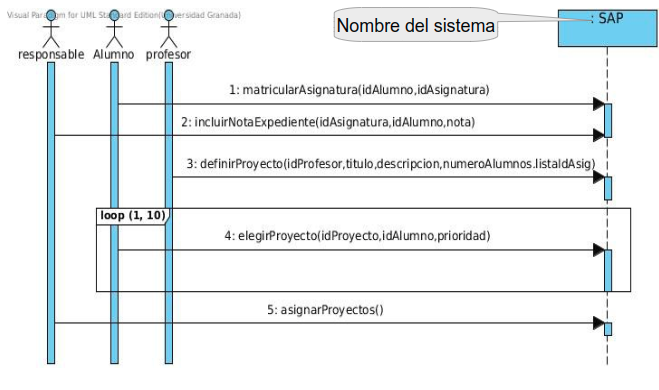
\includegraphics[scale=0.65]{ejemplo_dss.png}
\caption{Ejemplo de diagrama de secuencia.}
\end{figure}

\paragraph{Contratos.\\}

Un contrato es un documento que describe lo que una operación se propone lograr sin decir como se conseguirá. Es decir, define la especificación de una operación sin entrar en su implementación.\\

La plantilla de un contrato es la siguiente:

\begin{figure}[H]
\centering
\begin{tabular}{|m{7.5cm}|m{7.5cm}|}
\hline
\textbf{Nombre} & Nombre de la operación y sus parámetros.\\
\hline
\textbf{Responsabilidad} & Descripción informal de las responsabilidades que debe cumplir la operación.\\
\hline
\textbf{Tipo} & Concepto, clase o interfaz responsable de la operación. \\
\hline
\textbf{Notas} & Notas de diseño, algoritmo, etc.  \\
\hline
\textbf{Excepciones} & Casos excepcionales. \\
\hline
\textbf{Salida} & Mensajes o datos que proporciona.\\
\hline
\textbf{Precondiciones} & Suposición acerca del estado del sistema antes de ejecutar la operación.\\
\hline
\textbf{Poscondiciones} & Estado del sistema al terminar la operación. Creación y destrucción de objetos/enlaces, modificación de atributos, etc.\\
\hline
\end{tabular}
\caption{Plantilla de contrato.}
\end{figure}


\begin{figure}[H]
\centering
\begin{tabular}{|m{7.5cm}|m{7.5cm}|}
\hline
\textbf{Nombre} & \textbf{definirProyecto}(idProfesor,titulo,
descripcion,numeroAlumnas,listIdAsig)\\
\hline
\textbf{Responsabilidad} & Crea un nuevo proyecto inicializando su estado y asignándole el profesor que lo define y las asignaturas recomendadas.\\
\hline
\textbf{Tipo} & SAP\\
\hline
\textbf{Notas} &  \\
\hline
\textbf{Excepciones} & 
\begin{itemize}
	\item Si el profesor identificado por idProfesor no existe.
	\item Si algunas de las asignaturas identificadas por alguno de los elementos de listaIdAsig no existe.
\end{itemize} \\
\hline
\textbf{Salida} &\\
\hline
\textbf{Precondiciones} & \\
\hline
\textbf{Poscondiciones} & 
\begin{itemize}
	\item Fue creado un objeto, \emph{pro}, de la clase Proyecto debidamente inicializado.
	\item Fue creado un enlace entre \emph{pro} y el objeto Profesor, identificado por idProfesor.
	\item Para todos los elementos de 
	listaIdAsig:
	\item \quad Fue creado un enlace entre \emph{pro} y el objeto de la clase Asignatura identificado por el correspondiente elemento de listaIdAsig.
\end{itemize}
\\
\hline
\end{tabular}
\caption{Ejemplo de contrato.}
\end{figure}

\newpage

\section{Tema 3. Diseño e implementación}

\subsection{Introducción al diseño}

\subsubsection{Definición y características}

EL \textbf{diseño} es el proceso de aplicar distintos métodos, herramientas y principios con el propósito de definir un dispositivo, proceso o sistema con los suficientes detalles como para permitir su relización física.

\begin{figure}[H]
\centering
\includegraphics[scale=0.5]{diseno.png}
\caption{Diseño.}
\end{figure}

El \textbf{diseño del software} es el proceso de aplicar métodos, herramientas y principios de diseño para traducir el modelo de análisis a una representación del software que pueda ser codificada (modelo del diseño).

\begin{itemize}
	\item El diseño implica una \textbf{propuesta de solución} al problema especificado durante el análisis.
	\item Es una \textbf{actividad creativa} apoyada en la experiencia del diseñador.
	\item Está apoyado por principios, técnicas, herramientas, etc.
	\item Es una tarea \textbf{clave} para la calidad del producto software.
	\item Es la \textbf{base} para el resto de las etapas del desarrollo.
	\item Debe ser un proceso de \textbf{refinamiento}.
	\item El diseño garantiza que un programa funcione correctamente (\emph{hacer que un programa funcione $\neq$ hacer que funcione correctamente)}.
\end{itemize}

\subsubsection{Principios de diseño}

El diseño se basa en cuatro principios fundamentales: \textbf{modularidad}, \textbf{abstracción}, \textbf{ocultamiento de información} e \textbf{independencia modular}.


\paragraph{Modularidad\\}

Consiste en aplicar la estrategia \emph{divide y vencerás}. Un sistema software está formado por piezas (módulos) que encajan perfectamente e interactúan entre sí para llevar a cabo algún objetivo común.\\

Un \textbf{módulo sofware} es una unidad básica de descomposición de un sistema software y representa una entidad o funcionamiento específico. Pueden ser funciones, clases, paquetes, etc.\\

Las ventajas de la modularidad son:

\begin{itemize}
	\item Los módulos son más fáciles de documentar que todo el sistema.
	\item Facilitan los cambios.
	\item Reducen la complejidad.
	\item Son más fáciles de implementar.
	\item Posibilitan el desarrollo en paralelo.
	\item Permiten la prueba independiente.
	\item Facilitan el encapsulamiento.
\end{itemize}

\begin{figure}[H]
\centering
\includegraphics[scale=0.5]{modularidad_graf.png}
\caption{Gráfico adecuado de modularidad.}
\end{figure}

\paragraph{Abstracción\\}

Es un mecanismo que permite determinar lo que es relavante y lo que no en un nivel de detalle determinado, ayudando a obtener la modularidad necesaria para ese nivel de detalle.

\begin{figure}[H]
\centering
\includegraphics[scale=0.5]{abstraccion.png}
\caption{Abstracción.}
\end{figure}

Existen tres mecanismos fundamentales de abstracción en el diseño: \textbf{procedimental}, \textbf{de datos} y \textbf{de control}. \\

El proceso de ir incorporando detalles al diseño conforme vayamos bajando el nivel de abstracción se denomina \textbf{refinamiento}.

\begin{itemize}
	\item \textbf{Abstracción procedimental}. Consiste en abstraerse sobre el funcionamiento para conseguir una estructura modular basada en procedimientos (métodos).
	\begin{figure}[H]
	\centering
	\includegraphics[scale=0.5]{procedimental.png}
	\caption{Abstracción procedimental.}
	\end{figure}
	\item \textbf{Abstracción de datos}. Se abstrae tanto el funcionamiento como los atributos que definen el estado de una entidad, obteniendo una estructura modular basada en el estado y el funcionamiento de un objeto o entidad (se añaden variables).
	\begin{figure}[H]
	\centering
	\includegraphics[scale=0.5]{datos.png}
	\caption{Abstracción de datos.}
	\end{figure}
	\item \textbf{Abstracción de control}. Permikte abstraer sobre el flujo de control de cualquier proceso (definición de los métodos).
\end{itemize}

\paragraph{Ocultamiento de información\\}

Un módulo debe especificarse y diseñarse de forma que la información (procedimientos y datos) que está dentro del módulo sea inaccesible para otros módulos que no la necesiten.\\

Las ventajas del ocultamiento de información son:

\begin{itemize}
	\item Reduce la posibilidad de efectos colaterales.
	\item Limita el impacto global de las decisiones de diseño locales.
	\item Enfatiza la comunicación a través de interfaces controladas.
	\item Disminuye el uso de datos globales.
	\item Potencia la modularidad.
	\item Produce software de alta calidad.
\end{itemize}

\begin{figure}[H]
\centering
\includegraphics[scale=0.4]{ocultamiento.png}
\caption{Ocultamiento de información.}
\end{figure}

\paragraph{Independencia modular\\}

La independencia modular se mide en dos parámetros: \textbf{cohesión} y \textbf{acoplamiento}:

\begin{itemize}
	\item \textbf{Cohesión}. Grado que tiene un módulo en la realización de \emph{un solo objetivo}. Un módulo debe presentar un alto nivel de cohesión, ya que hace que sea más fácil de entender, reutilizar y mantener.
	\item \textbf{Acoplamiento}. Mide la interdependencia entre módulos dentro de una estructura de software. Un módulo debe presentar un nivel de acoplamiento lo más bajo posible con respecto a los demás módulos. 
\end{itemize}

\subsubsection{Herramientas de diseño}

Las \textbf{herramientas de diseño} son los instrumentos que ayudan a representar los modelos de diseño del software. Algunas de las más usadas son:
\begin{itemize}
	\item Diagramas UML (de clase, de interacción, de paquetes, etc.).
	\item Cartas de estructura.
	\item Tablas de decisión.
	\item Diagramas de flujo de control.
	\item Lenguajes de diseño de programas (LDP).
\end{itemize}
\newpage
\subsubsection{Métodos de diseño}

Un \textbf{método de diseño} permite obtener diseños de forma sistemática, proporcionando las herramientas, técnicas y pasos a seguir para llevar a cabo del diseño. Todo método de diseño debe poseer:
\begin{itemize}
	\item \textbf{Principios} en los que se basa.
	\item \textbf{Mecanismos de traducción} del modelo de análisis al modelo de diseño.
	\item \textbf{Herramientas} que nos permitan refinar el diseño.
	\item Criterios para \textbf{evaluar} la calidad del diseño.
\end{itemize}

\subsubsection{Modelo de diseño}


A nivel general un modelo de diseño está formado por varios \textbf{subsistemas} de diseño junto con las interfaces que requieren o proporcionan estos subsistemas. A su vez, cada subsistema puede contener distintos tipos de elementos de modelado de diseño, principalmente \emph{realización de casos de uso-diseño} y \emph{clases de diseño}.


\begin{figure}[H]
\centering
\begin{subfigure}[b]{0.5\textwidth}
\includegraphics[width=\textwidth]{modelo_diseno.png}
\end{subfigure}
\quad
\begin{subfigure}[b]{0.45\textwidth}
\includegraphics[width=\textwidth]{modelo_diseno_2.png}
\end{subfigure}
\caption{Modelo de diseño.}
\end{figure}

El modelo de diseño puede considerarse un refinamiento del modelo de análisis en el que todos los artefactos de éste están mejor definidos e incorporan detalles técnicos que permiten su implementación.

\begin{figure}[H]
\centering
\begin{tabular}{|m{7cm}|m{7cm}|}
\hline
\textbf{Estrategia} & \textbf{Consecuencias}\\
\hline
Modificar el modelo de análisis. & Se tiene solo un modelo pero se pierde la vista del análisis.\\
\hline
Modificar el modelo de análisis y usar una herramienta que recupere el original & Se tiene un solo modelo, pero la vista recuperada puede no ser satisfactoria.\\
\hline
Congelar el modelo de análisis y hacer una copia para continuar con el diseño. & Se tienen dos modelos que no van al mismo ritmo.\\
\hline
Mantener ambos modelos. & Se tienen dos modelos al mismo tiempo, pero hay sobrecarga de mantenimiento.\\
\hline
\end{tabular}
\caption{Paso de modelo de análisis a modelo de diseño.}
\end{figure}

\begin{figure}[H]
\centering
\includegraphics[scale=0.75]{correspondencia_analisis_diseno.png}
\caption{Correspondencia entre modelo de análisis y de diseño.}
\end{figure}

\subsubsection{Tareas del diseño}

\begin{figure}[H]
\centering
\includegraphics[scale=0.75]{tareas_diseno.png}
\caption{Tareas del diseño.}
\end{figure}

\subsection{Diseño de los casos de uso}


\subsubsection{Modelo de interacción de objetos}

Las herramientas para representar el modelo son los diagramas de interacción UML: el de \textbf{secuencia} y el de \textbf{comunicación}. Son semánticamente equivalentes.

\subsubsection{Patrones de diseño de Craig Larman}

Resuelven el problema de la asignación de responsabilidades a objetos.\\

Una responsabilidad es una obligación que debe tener un objeto en su comportamiento. Todas ellas deben incluirse en alguna operación o método de la clase a la que pertenece el objeto. Las responsabilidades de un objeto pueden ser:

\begin{itemize}
	\item \textbf{Conocer}: datos privados encapsulados en él, objetos relacionados con él, cálculos que puede hacer, etc.
	\item \textbf{Hacer}: iniciar una acción sobre sí mismo o sobre otro objeto, controlar y coordinar actividades entre objetos, etc.
\end{itemize}

Los \textbf{patrones de diseño de Craig Larman} sirven como ayuda para encontrar estas responsabilidades.\\

Un \textbf{patrón de diseño} es la descripción de un problema con su solución en un contexto determinado. Sus pares importantes son:

\begin{itemize}
	\item Su \textbf{nombre}.
	\item El \textbf{problema} que pretende solucionar.
	\item La \textbf{solución} propuesta.
	\item Las \textbf{consecuencias} buenas y malas que puede ocasionar su uso.
\end{itemize}

Los patrones Craig Larman son varios: \textbf{experto en información}, \textbf{creador}, \textbf{controlador}, \textbf{bajo acoplamiento}, \textbf{alta cohesión}, polimorfismo, etc.

\begin{figure}[H]
\centering
\begin{tabular}{|m{5cm}|m{8cm}|}
\hline
\textbf{Nombre} & Experto en información\\
\hline
\textbf{Problema} & Complejidad en la búsqueda de información y acoplamientos fuertes entre clases en las búsquedas.\\
\hline
\textbf{Solución} & Asignar responsabilidad a la clase que contiene la información necesaria.\\
\hline
\textbf{Consecuencias} & 
\begin{itemize}
	\item \textbf{Buenas}: mantiene el ocultamiento de información y distribuye el comportamiento.
	\item \textbf{Malas}: en ocasiones va en contra de los principios de acoplamiento o cohesión.
\end{itemize}\\
\hline
\end{tabular}
\caption{Patrón experto en información}
\end{figure}

\begin{figure}[H]
\centering
\includegraphics[scale=0.75]{experto_inf.png}
\caption{Ejemplo de patrón experto en información.}
\end{figure}

\begin{figure}[H]
\centering
\begin{tabular}{|m{5cm}|m{8cm}|}
\hline
\textbf{Nombre} & Creador\\
\hline
\textbf{Problema} & Tener acoplamientos, mala encapsulación y reutilización y poca claridad en la construcción de objetos.\\
\hline
\textbf{Solución} & Asignar a la clase B la responsabilidad de crear una instancia de A en caso de que agregue, contenga, registre, utilice o tenga los datos de inicialización de A\\
\hline
\textbf{Consecuencias} & 
\begin{itemize}
	\item \textbf{Buenas}: produce bajo acoplamiento.
	\item \textbf{Malas}: no es conveniente usarlo cuando las instancias ya existen.
\end{itemize}\\
\hline
\end{tabular}
\caption{Patrón creador}
\end{figure}

\begin{figure}[H]
\centering
\includegraphics[scale=0.75]{ej_creador.png}
\caption{Ejemplo de patrón creador.}
\end{figure}

\begin{figure}[H]
\centering
\begin{tabular}{|m{5cm}|m{8cm}|}
\hline
\textbf{Nombre} & Bajo acoplamiento\\
\hline
\textbf{Problema} & Elementos que dependen de demasiados elementos. Una modificación conlleva demasiadas modificaciones colaterales.\\
\hline
\textbf{Solución} & Asignar responsabilidades de forma que tengamos elementos que dependan sólo de los elementos necesarios.\\
\hline
\textbf{Consecuencias} & 
\begin{itemize}
	\item \textbf{Buenas}: no afectan los cambios en otros elementos, son fáciles de entender de manera aislada y aumenta la reutilización.
	\item \textbf{Malas}: si se lleva a un extremo puede ocasionar diseños pobres. El nivel de acoplamiento debe ser adecuado.
\end{itemize}\\
\hline
\end{tabular}
\caption{Patrón de bajo acoplamiento}
\end{figure}

\begin{figure}[H]
\centering
\begin{tabular}{|m{5cm}|m{8cm}|}
\hline
\textbf{Nombre} & Alta cohesión\\
\hline
\textbf{Problema} & Elementos con pocas tareas o con muchas pero no relacionadas. \\
\hline
\textbf{Solución} & Asignar responsabildiades de forma que todas las tareas de un elemento persigan un objetivo común.\\
\hline
\textbf{Consecuencias} & 
\begin{itemize}
	\item \textbf{Buenas}: el diseño es más claro, se simplifica el mantenimiento y aumenta la reutilización.
	\item \textbf{Malas}: ninguna, sólo debemos renunciar a este patrón cuando haya un motivo de peso. 
\end{itemize}\\
\hline
\end{tabular}
\caption{Patrón de alta cohesión}
\end{figure}

\begin{figure}[H]
\centering
\includegraphics[scale=0.7]{ej_alta_cohesion.png}
\caption{Ejemplo de patrón de alta cohesión.}
\end{figure}

\begin{figure}[H]
\centering
\begin{tabular}{|m{5cm}|m{8cm}|}
\hline
\textbf{Nombre} & Controlador o fachada\\
\hline
\textbf{Problema} & Comunicación entre los objetos de la capa del dominio de la solución y la capa de la interfaz.\\
\hline
\textbf{Solución} & Asignar responsabilidades de recibir o manejar un mensaje de evento del sistema a una clase que representa al sistema global o bien al caso de uso (un controlador por cada caso de uso).\\
\hline
\textbf{Consecuencias} & 
\begin{itemize}
	\item \textbf{Buenas}: se asegura que la lógica de la aplicación no se maneja en la interfaz. Buena reutilización y bajo nivel de acoplamiento. Permite razonar sobre el estado de los casos de uso.
	\item \textbf{Malas}: Controladores saturados.
\end{itemize}\\
\hline
\end{tabular}
\caption{Patrón controlador o fachada}
\end{figure}

\subsubsection{Elaboración del modelo de interacción de objetos}

\begin{itemize}
	\item Las bases principales para obtener los diagramas de comunicación son los contratos y el modelo conceptual.
	\item El modelo conceptual sirve como guía para saber qué objetos pueden interactuar en una operación.
	\item Todo lo especificado en el contrato debe satisfacerse en el diagrama correspondiente.
	\item Para elaborar cada diagrama podemos ayudarnos de los patrones de diseño de Craig Larman.
\end{itemize}

Los pasos a seguir son los siguientes:

\begin{enumerate}
	\item Elaborar los diagramas de interacción teniendo en cuenta el diagrama de conceptos y el contrato asociado.
	\item Inicializar el sistema.
	\item Establecer las relaciones entre el modelo y la interfaz de usuario.
\end{enumerate}



\subsection{Diseño de la estructura de clases}


\subsubsection{Modelo de estructura de objetos: diagrama de clases del diseño}

Un diagrama de clases del diseño describe gráficamente las especificaciones de las clases e interfaces software y las relaciones entre éstas en una aplicación. A diferencia del modelo conceptual, representa la solución a nuestro problema. Puede contener los siguientes elementos:
\begin{itemize}
	\item Clases con sus atributos y sus operaciones.
	\item Interfaces con sus operaciones y constantes.
	\item Relaciones entre clases, interfaces o clases e interfaces.
	\item Información sobre el tipo de los atributos y parámetros.
	\item Navegabilidad de las asociaciones.
\end{itemize}

Se representan mediante un diagrama de clases UML.\\

\subsubsection{Proceso de elaboración del diagrama de clases del diseño}

Los pasos a seguir para elaborar el diagrama son los siguientes:

\begin{enumerate}
	\item Identificar y representar las clases. Todos los objetos de los diagramas comunicación tendrán su correspondiente clase. Tomarán los atributos del modelo conceptual ey de los diagramas de comunicación.
	\item Añadir las operaciones. Todos los envíos de mensajes deben tener su operación en la clase correspondiente.
	\item Añadir los tipos de atributos y los parámetros.
	\item Incluir las asociaciones y la navegabilidad.
	\item Incluir las dependencias.
\end{enumerate}

\subsection{Diseño de la arquitectura}


\subsubsection{Conceptos de diseño de la arquitectura}

El \textbf{diseño de la arquitectura} proporcionará una imagen global de la estructura del sistema software, esbozando los artefactos más importantes que lo componen (principalmente subsistemas y sus interfaces).\\

Determinar la arquitectura del software consiste en tomar decisiones respecto a:
\begin{itemize}
	\item Cómo se dividirá el sistema en subsistemas.
	\item Cómo deberán interactuar dichos subsistemas.
	\item Cuál será la interfaz de cada subsistema.
	\item Cuándo será el estilo arquitectónico usado.
\end{itemize}

La arquitectura es muy importante debido a que:
\begin{itemize}
	\item Facilita la comprensión de la estructura global del sistema.
	\item Permite trabajar en los subsistemas de forma independiente.
	\item Facilita las posibles extensiones del sistema.
	\item Facilita la reutilización de los distintos subsistemas.
\end{itemize}


\subsubsection{Herramientas para su representación}

\begin{itemize}
	\item \textbf{Diagrama de paquetes}. Describe el sistema en torno a agrupaciones lógicas y proporciona una primera estructura.
	\item \textbf{Diagrama de compontentes}. Representa una estructuración concreta del sistema a partir de los sistemas (componentes software) y su correspondiente interfaz (interrelación)
	\item \textbf{Diagrama de despliegue}. Especifica el hardware físico sobre el que se ejecutará el sistema software y cómo cada uno de los subsistemas software se despliega en ese hardware.
\end{itemize}


\subsubsection{Estilos arquitectónicos}

Un estilo arquitectónico proporciona un conjunto de subsistemas predefinidos, especificando sus responsabilidades e incluyendo reglas y guías para organizar las relaciones entre ellos. No proporcionan la arquitectura del sistema, sino una guía para obtenerla.

\paragraph{Arquitectura multicapa\\}

Distribuye los subsistemas en capas, de forma que:
\begin{itemize}
	\item Cada capa presta servicios a la capa superior y actúa como cliente sobre las capas más internas.
	\item El diseño incluye los protocolos que establecen cómo interactuará cada par de capas.
	\item Las capas más claras proporcionan servicio de bajo nivel (comunicación en red, acceso a bases de datos, etc.)
\end{itemize}

Sus principales ventajas son:

\begin{itemize}
	\item Cada capa puede diseñarse, implementarse y probarse de forma independiente.
	\item La arquitectura es fácilmente portable: podemos cambiar una capa si mantenemos la interfaz y los cambios en la interfaz sólo afectan a la capa adyacente.
\end{itemize}

Sus principales ventajas son la dificultad para determinar los servicios de cada capa y la pérdida de rendimiento debida a los múltiples niveles que hay que pasar para completar una petición.

\begin{figure}[H]
\centering
\includegraphics[scale=0.6]{multicapa.png}
\caption{Arquitectura multicapa.}
\end{figure}

\begin{itemize}
	\item Las capas pueden diseñarse, construirse y probarse de forma \textbf{independiente}.
	\item Una capa bien diseñada tiene \textbf{alta cohesión}.
	\item Las capas deben estar lo más desacopladas posible.
	\item Una capa de un nivel no debe tener conocimiento de las capas superiores (\textbf{ocultamiento de información}).
	\item Las capas más inferiores deben prestar servicios de bajo nivel (\textbf{bajo acoplamiento}).
\end{itemize}

\paragraph{Arquitectura cliente-servidor\\}

Están compuestas por:

\begin{itemize}
	\item \textbf{Servidores} independientes que ofrecen servicios a otros subsistemas.
	\item \textbf{Clientes} que pueden solicitar estos servicios.
	\item \textbf{Red} que permite a los clientes realizar peticiones a los servidores.
\end{itemize}

\begin{figure}[H]
\centering
\includegraphics[scale=0.75]{cliente-servidor.png}
\caption{Arquitectura cliente-servidor.}
\end{figure}

Las capas fundamentales son: de presentación (\textbf{clientes}) y procesamiento de aplicación y administración de datos (\textbf{servidores}).

\begin{itemize}
	\item la descomposición en clientes y servidores permite realizar el diseño de ambas partes de forma \textbf{independiente}.
	\item Mejora la \textbf{cohesión} de los subsistemas al proporcionar servicios específicos a los clientes.
	\item Reduce el \textbf{acoplamiento} al establecer la red de comunicación.
	\item Aumenta el nivel de \textbf{abstracción} al tener subsistemas o componentes distribuidos en nodos separados.
	\item Facilita la \textbf{reutilización}.
	\item Los sistemas distribuidos pueden \textbf{reconfigurarse fácilmente} añadiendo servidores o clientes extras.
	 \item Pueden escribirse clientes para nuevas plataformas sin modificar los servidores.
\end{itemize}

\paragraph{Arquitectura de repositorio\\}

Los datos se ubican en una base de datos central a la que acceden todos los subsistemas. Los repositorios pueden ser activos o pasivos.

\begin{figure}[H]
\centering
\includegraphics[scale=0.5]{repositorio.png}
\caption{Arquitectura de repositorio.}
\end{figure}

Sus principales ventajas son:

\begin{itemize}
	\item Es una forma eficiente de compartir grandes cantidades de datos.
	\item Los subsistemas productores de datos no necesitan saber de los consumidores.
	\item Seguridad, control de acceso y recuperación de datos están centralizadas.
\end{itemize}

Sus inconvenientes son:

\begin{itemize}
	\item Todos los subsistemas deben estar acordes con el modelo de depósito. Es difícil integrar nuevos subsistemas.
	\item Es difícil evolucionar hacia otro modelo de datos.
	\item Fuerza la política de seguridad, control de acceso y recuperación de los subsistemas.
\end{itemize}

\begin{itemize}
	\item Se pueden diseñar subsistemas independientes, aunque deben conocer el esquema de los datos del repositorio.
	\item Mejora la \textbf{cohesión} de los subsistemas.
	\item El \textbf{acoplamiento} es alto, haciendo difíciles los cambios.
\end{itemize}

\newpage

\paragraph{Arquitectura MVC\\}

Consta de tres componentes, cada uno con un contenido determinado:

\begin{itemize}
	\item \textbf{Modelo}. Responsable del conocimiento del dominio de la aplicación.
	\item \textbf{Vista}. Responsable de mostrar los objetos del dominio de aplicación al usuario.
	\item \textbf{Controlador}. Responde a las acciones del usuario, invocando peticiones al modelo y a la vista.
\end{itemize}

\begin{figure}[H]
\centering
\includegraphics[scale=0.75]{mvc.png}
\caption{Arquitectura MVC.}
\end{figure}

\begin{itemize}
	\item Cada subsistema puede diseñarse de forma \textbf{independiente}.
	\item Se puede aumentar la \textbf{cohesión} si la vista y el controlador se encuentran unidos en una capa de interfaz de usuario.
	\item Se reduce el \textbf{acoplamiento}.
	\item La vista y el controlador hacen uso extensivo de componentes \textbf{reutilizables}.
	\item Es \textbf{flexible}: se puede modificar la interfaz de usuario cambiando la vista, el controlador o ambos.
	\item Se puede probar la aplicación separadamente de la interfaz de usuario.
\end{itemize}

\newpage

\paragraph{Arquitectura MDA (\textit{Modern Driven Architecture}\\}

Permite organizar y gestionar las arquitecturas empresariales. Está basado en herramientas automáticas para construir modelos independientes y transformarlos en implementaciones eficientes.\\

Los modelos son:

\begin{itemize}
	\item \textbf{CIM} (\textit{Computation Independent Model}). Se encarga del modelado de negocio y requisitos.
	\item \textbf{PIM} (\textit{Platform Independent Model}).
		\begin{itemize}
			\item Análisis y diseño independiente de la plataforma tecnológica.
			\item El analista realiza el PIM que describe al sistema.
			\item Un PIM se transforma en uno o varios PSM.
		\end{itemize}
		\item \textbf{PSM} (\textit{Platform Dependent Model}).
			\begin{itemize}
			\item Análisis y diseño dependiente de la plataforma tecnológica.
			\item El arquitecto adapta el modelo para una implementación tecnológica específica.
			\item Cada PSM se transforma en código.
		\end{itemize}
\end{itemize}

\subsubsection{Actividades del diseño arquitectónico}

Las actividades del diseño arquitectónico son:

\begin{enumerate}
	\item \textbf{Identificar objetivos}.
	\item \textbf{Determinar y modelar la arquitectura software y los subsistemas}.
	\item \textbf{Modelar la arquitectura software}.
	\item \textbf{Refinar la descomposición en subsistemas}.
\end{enumerate}

\paragraph{Identificar objetivos\\}

\begin{itemize}
	\item Se identifican las cualidades deseables del sistema que determinarán el diseño del mismo.
	\item Se obtienen a partir de los requisitos no funcionales o del dominio de la aplicación.
	\item Se selecciona un pequeño conjunto de objetivos que el sistema deberá satisfacer necesariamente.
	\item Se adquieren compromisos, ya que muchos objetivos de diseño son contrapuestos.
\end{itemize}

\paragraph{Determinar y modelar la arquitectura\\}

Para \textbf{determinarla} hay que:

\begin{itemize}
	\item Seleccionar el estilo arquitectónico adecuado.
	\item Identificar subsistemas.
	\item Añadir subsistemas predefinidos por el estilo arquitectónico elegido.
\end{itemize}

Para \textbf{modelarla} hay que:

\begin{itemize}
	\item Diseñar la arquitectura en un diagrama de paquetes.
	\item Elaborar el diagrama de componentes de la vista de arquitectura.
	\item Realizar el diagrama de despliegue.
\end{itemize}

\paragraph{Modelar la arquitectura software\\}

Para modelar se utilizan dos tipos de diagramas:

\begin{itemize}
	\item \textbf{Diagrama de paquetes}. Permite modelar una primera estructuración o partición del sistema en base a uno o más paquetes.
	\item \textbf{Diagrama de componentes}. Permite estructurar el sistema en subsistemas en base a componentes que pueden reemplazarse.
\end{itemize}

\paragraph{Refinar la descomposición en subsistemas\\}

Consiste en refinar los subsistemas hasta satisfacer los objetivos del diseño. Se establecen los siguientes aspectos genéricos:

\begin{itemize}
	\item Correspondencia hardware-software.
	\item Administración de datos persistentes.
	\item Especificación de una política de control de accesos.
	\item Diseño del flujo de control.
	\item Diseño de la concurrencia y sincronización.
	\item Definición de las condiciones del entorno.
\end{itemize}


\end{document}